\documentclass{wmnotes}

\lecture{Naturwissenschaftliche Grundlagen der Medizin}
\subtitle{Physik für Mediziner}
\professor{Prof. Jürg Osterwalder}
\semester{HS 2011}
\author{Michal Sudwoj}
\authoremail{michal.sudwoj@uzh.ch}

\begin{document}

\part{Vorlesungsnotizen}
\setcounter{chapter}{-1}
\chapter{Wozu Physik für Mediziner?}
Physik = Lehre der Naturgesetze
\begin{enumerate}
	\item Mensch \& Tier: Teil der Natur $\rightarrow$ Verständnis des Organismus
		\begin{bsp*}
			\begin{itemize}
				\item Hüftgelenk $\rightarrow$ Mechanik, Festigkeitslehre
				\item Auge $\rightarrow$ Optik
				\item Reizübertragung (Nerven) $\rightarrow$ Elekrizität
				\item Blutzirkulation $\rightarrow$ Strömungslehre
			\end{itemize}
		\end{bsp*}
	\item Diagnostik-/Therapiewerkzeuge $\rightarrow$ physikalische Apparate
		\begin{bsp*}
			\begin{itemize}
				\item Röntgenapparatur, CT, MRI $\rightarrow$ Verstehen der Resultate $\rightarrow$ Schutz von Patient + Personal
			\end{itemize}
		\end{bsp*}
	\item Besondere Berufsbilder
		\begin{itemize}
			\item Gerichtsmediziner
			\item Sicherheit, Unfallverhütung
			\item Strahlenschutz
		\end{itemize}
	\item Analytisches Denken! Probleme lösen: (Diagnose, Entscheidungen treffen)
\end{enumerate}
\chapter{Mechanik}

\section{Kinematik}
Beschreibung von Bewegungen \\
einfachster Fall:
\begin{itemize}
	\item geradlinige Bahn (1D)
	\item gleichförmige Bewegung
\end{itemize}
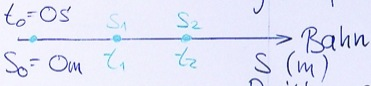
\includegraphics{Bild1}

\subsection{Weg-Zeit-Diagramm}
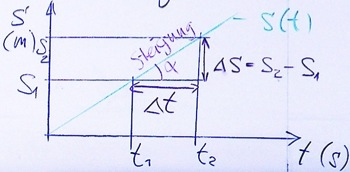
\includegraphics{Bild2}
\[ \tan \alpha = \frac{\Delta s}{\Delta t} \overset{!}{=} v \]
konst. Steigung von $s(t) \implies$ konst. $v$

\subsection{Geschwindigkeit}
\begin{def*}[ note = Geschwindigkeit , index = Geschwindigkeit ]
	\[
		v = \frac{\Delta s}{\Delta t} \\
		[v] = \frac{m}{s}
	\]
\end{def*}

\subsection{Geschwindigkeits-Zeit Diagramm}
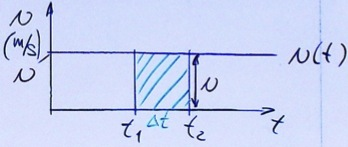
\includegraphics{Bild3}
\[
	v(t) = \frac{\Delta s}{\Delta t} \\
	\text{Fläche} = v \cdot \Delta t = \Delta s \text{ ! } = \text{ zurückgelegter Weg}
\]

\subsection{Nicht-gleichförmige Bewegungen}
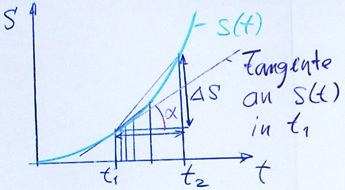
\includegraphics{Bild4}
Geschwindigkeit $v(t)$
\[
	\overline{v} = \frac{\Delta s}{\Delta t} = \text{ mittlere Geschwindigkeit zw. $t_1$ und $t_2$} \\
	v(t_1) = \lim_{t_1 \rightarrow t_2} \frac{\Delta s}{\Delta t} \underset{\text{\scriptsize{Math.}}}{=} s'(t) \\
	v(t) = s'(t) \\
\]

\subsubsection{Schreibweise}
\[
	\Delta t \rightsquigarrow \dd t \\
	v(t) = s'(t) \eqqcolon \frac{\dd s}{\dd t}
\]
1. Ableitung \\
$v(t)$: Momentangeschwindigkeit
\begin{bsp*}[ note = $v$ nimmt gleichmässig zu ]
	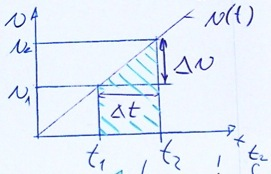
\includegraphics{Bild5}
	\[ \text{Fläche } \underset{\text{\scriptsize{Math.}}}{\overset{\text{!}}{=}} \int_{t_1}^{t_2} v(t) \dd t \]
\end{bsp*}
\todo{Undefined seq.}
Änderung der Geschwindigkeit mit der Zeit:
\begin{def*}[ note = Beschleunigung , index = Beschleunigung ]
	\[
		a = \frac{\Delta v}{\Delta t} \\
		[a] = \frac{m}{s^2}
	\]
\end{def*}
Fall:
\begin{itemize}
	\item gleichförmige Beschleunigung: $a =$ konst.
	\item beliebige Funktion $a(t)$
\end{itemize}
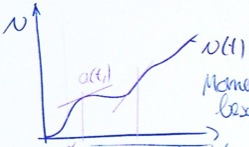
\includegraphics{Bild6} \\
analog:
\[
	a(t) = \frac{\dd v}{\dd t} \\
	a(t) = \frac{\dd}{\dd t} \left( \frac{\dd s}{\dd t} \right) = s''(t) \eqqcolon \frac{\dd^2 s}{\dd t^2}
\]

\begin{rep*}[note = Kinematik (1D-Fall)]
	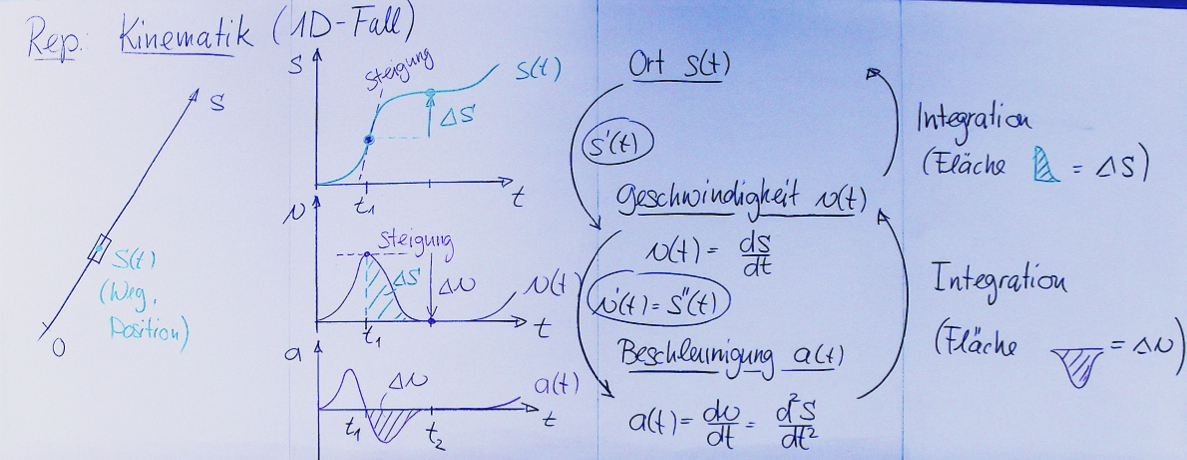
\includegraphics[ width = \textwidth ]{Bild7}
\end{rep*}
\begin{bsp*}[note = Der freie Fall]
	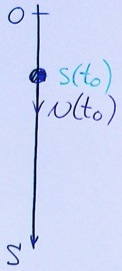
\includegraphics{Bild8} \\
	auf der Erdoberfläche
	\[ a(t) = a_{\text{Fall}} = g = 9.81 \frac{\text{m}}{{\text{s}}^2} \]
	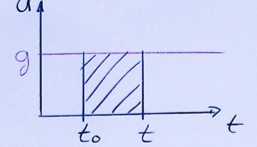
\includegraphics{Bild9}
	\[ \text{Fläche } = g( t - t_0 ) \]
	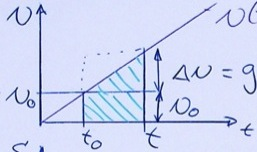
\includegraphics{Bild10}
	\[
		v(t) = v_0 + g( t - t_0 ) \\
		\Delta v = g( t - t_0 ) \
		\text{Fläche } = v_0 ( t - t_0 ) + \frac{1}{2} g( t - t_0 )^2 = \Delta S
	\]
	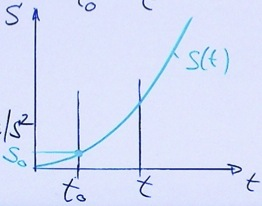
\includegraphics{Bild11}
	\[ s(t) = s_0 + v_0 ( t - t_0 ) + \frac{1}{2} g( t - t_0 ) \]
	
	einfachster Fall:
	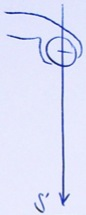
\includegraphics{Bild12}
	\[
		s(0) = 0 \\
		t_0 = 0 \\
		s_0 = 0 \\
		v_0 = 0 \\
		\implies s(t) = \frac{1}{2} gt^2
	\]
\end{bsp*}

\subsection{Bewegungen in der Ebene}
\subsubsection{Ortsvektor \texorpdfstring{$\vec{r}(t)$}{r(t)}}
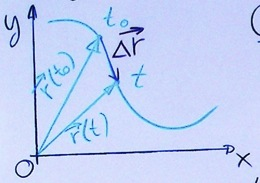
\includegraphics{Bild13}
\begin{itemize}[label = $\rightarrow$]
	\item Länge (Betrag)
	\item Richtung
\end{itemize}

Geschwindigkeit: $\frac{\text{Weg}}{\text{Zeit}}$
Weg: $\Delta \vec{r} = \vec{r}(t) - \vec{r}(t_0)$ \\
$\vec{v} = \frac{\Delta \vec{r}}{\Delta t}$ mittlere Geschwindigkeit \\
Momentangeschwindigkeit: $\vec{v}(t) = \lim_{\Delta t \rightarrow 0} \frac{\Delta \vec{r}}{\Delta t} \overset{\text{\scriptsize{Math.}}}{=} \frac{\dd \vec{r}}{\dd t}$ \\
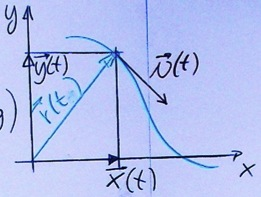
\includegraphics{Bild14}
\[
	\vec{r}(t) = \vec{x}(t) + \vec{y}(t) \\
	\implies \text{ Komponentenschreibweise} \\
	\vec{r}(t) = ( x(t) , y(t) ) \\
	\frac{\dd \vec{r}}{\dd t} = \left( \frac{\dd x}{\dd t} , \frac{\dd y}{\dd t} \right)
\]
$v(t)$:
\begin{itemize}
	\item Betrag (Schnelligkeit)
	\item Richtung! (tangential zu Bahn)
\end{itemize}
\subsubsection{Schnelligkeit}
\[ \abs{\vec{v}(t)} = v(t) = \sqrt{{v_1}^2(t) + {v_2}^2(t)} \]
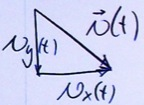
\includegraphics{Bild15}

\subsubsection{Momentanbeschleunigung}
\[ \vec{a}(t) = \frac{\dd \vec{v}}{\dd t} = \frac{\dd^2 \vec{s}}{\dd t^2} \]

\subsection{Wann ist eine Bewegung beschleunigt?}
Wenn $\vec{v}$ sich ändert!
\begin{itemize}[label = $\rightarrow$]
	\item Betrag
	\item Richtung!
\end{itemize}
\begin{bsp*}[note = Kreisbewegung mit konstante Umlaufgeschwindigkeit]
	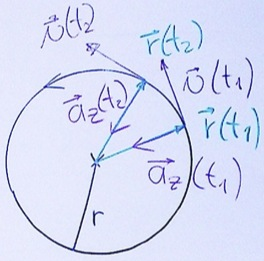
\includegraphics{Bild16}\\
	$\implies v =$ konst., $\vec{v}$ dreht $\implies$ Zentripetalbeschleunigung
	\[ a = \frac{v^2}{r} \]
\end{bsp*}
\begin{bsp*}[note = beliebige Kreisbewegung ($v \neq$ konst.)]
	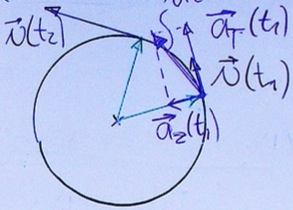
\includegraphics{Bild17} \\
	\[ \begin{matrix*}[l]
		a_Z(t) = \frac{v^2(t)}{r}		&\text{Zentripetalbeschleunigung} \\
		a_T(t) = \frac{\dd v}{\dd t}	&\text{Tangentialbeschleunigung}
	\end{matrix*} \]
\end{bsp*}

\subsection{Bewegungen im 3D-Raum}
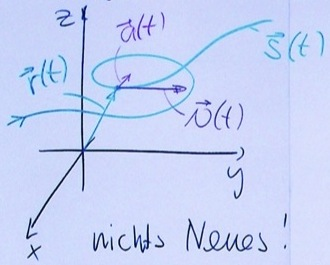
\includegraphics{Bild18} \\
nicht Neues!
\[ \vec{r}(t) = ( x(t) , y(t) , z(t) ) \]

\section{Dynamik}
$\implies$ Ursache der Bewegung
\subsection{Kraft/Masse}
\begin{def*}[ note = Kraft , index = Kraft ]
	\dots Wirkung!
\end{def*}
\begin{bsp*}
	\begin{itemize}
		\item Gewicht heben
		\item Deformation (Messung!)
		\item Bewegung
	\end{itemize}
\end{bsp*}
\begin{def*}[ note = Masse , index = Masse ]
	\enquote{Trägheit} (\enquote{\dots schwieriger in Bewegung zu setzen})
\end{def*}
Kraft: Vektor! \\
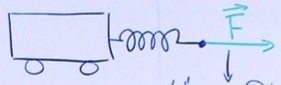
\includegraphics{Bild19} \\
Länge, Richtung, Angriffspunkt

\subsection{Die Newtonschen Prinzipien (1686)}
\begin{gather*}
	\underbrace{\vec{F}}_{\text{Ursache}} = \underbrace{m \cdot \vec{a}}_{\text{Wirkung}} \\
	[F] = \si{\kilo\gram\metre\per\second\tothe{2}} = \si{\newton} \quad ( \text{Newton} )
\end{gather*}
$\implies$ 2. Newtonsche Prinzip (Axiom) (Aktionsprinzip) \\
Anwendung: \\
\begin{itemize}
	\item Mann kennt Kraft $\implies$ Beschleunigung + Bahn berechnen
	\item Ich sehe Beschleunigung $\implies$ Was für Kräfte wirken
\end{itemize}
\subsubsection{1. Newtonsches Prinzip (Trägheitsprinzip)}
kräftefreie Körper ( $\vec{F} = \vec{0}$ , $\sum_i \vec{F_i} = \vec{0}$ )
\begin{itemize}[ label = $\rightarrow$ ]
	\item Körper in Ruhe (ist + bleibt)
	\item bewegt sich mit konst. Geschwindigkeit $\vec{v} =$ konst.
\end{itemize}
$\implies$ Bewegungszustände

\subsubsection{Newtonsches Prinzip (Reaktionsprinzip)}
(action = reactio) \\
Kräfte rühren immer von Wechselwirkungen (WW)
\begin{bsp*}[note = Feder]
	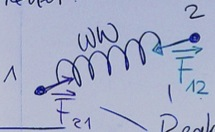
\includegraphics{Bild20}
	\[ \vec{F_{21}} = -\vec{F_{12}} \]
	Reaktionspartner $\rightarrow$ greifen immer an verschiedenen Körper an
\end{bsp*}
\begin{rep*}[ note = Dynamik ]
	Kraft: erzeugt Bewegung \\
	Masse: Trägheit \\
	Newtonsche Prinzipien \\
	\begin{enumerate}
		\item kräftefreier Körper: $\vec{v} =$ konst. (z.B. $\vec{v} = \vec{0}$)
		\item $\vec{F} = m \vec{a}$ Ursache \& Wirkung
		\item Kräfte rühren \textbf{immer} von WW her \\
			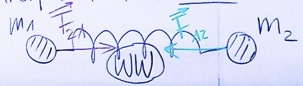
\includegraphics{Bild21} \\
			$\vec{F_{21}} = -\vec{F_12}$
	\end{enumerate}
\end{rep*}
\begin{bsp*}[ note = Hammer \& Nagel ]
	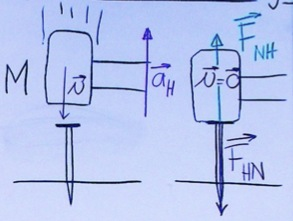
\includegraphics{Bild22}
	\begin{enumerate}[start = 2]
		\item $\vec{F_{NH}} = M \vec{a_H}$
		\item $\vec{F_HN} = -\vec{F_{NH}}$
	\end{enumerate}
\end{bsp*}

\subsection{Arten von Kräften}
\subsubsection{Gravitationskraft}
(Anziehung von Massen) \\
auf Erdoberfläche Gewichtskraft $\vec{G}$ \\
\begin{tabular}{ll}
	Betrag:			&$mg$ \\
	Richtung:			&zum Erdmittelpunkt \\
	Angriffspunkt:	&Schwerpunkt \\
	Reaktionspartner:	&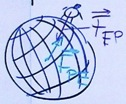
\includegraphics{Bild23}
\end{tabular}

\subsubsection{Elektromagnetische Kräfte}
(Anziehung / Abstossung von Ladungen)
\begin{itemize}[ label = $\rightarrow$ ]
	\item Coulombkraft (elektrische Kraft; verschiedene Erscheingungsformen)
	\item magnetische Kraft
	\item Lorentzkraft
\end{itemize}

\subsubsection{starke Kraft}
\begin{itemize}[ label = $\rightarrow$ ]
	\item Stabilität der Atomkeime
\end{itemize}

\subsubsection{schwache Kraft}
\begin{itemize}[ label = $\rightarrow$ ]
	\item Radioaktivität
\end{itemize}

\subsection{Coulombkraft und ihre Erscheinungsformen}
\begin{itemize}
	\item elastische Kräfte im festen Körpern (Kohäsion)
	\item Berührungskräfte - Die Normalkraft
		\begin{bsp*}[ note = Quader auf Tisch in Ruhe ]
			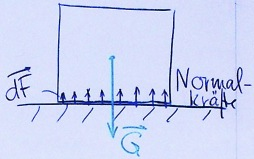
\includegraphics{Bild24}
			\begin{gather*}
				\sum \vec{F_a} = \vec{0} \\
				\implies \vec{G} + \sum \vec{\dd F} = \vec{0}
			\end{gather*}
		\end{bsp*}
\end{itemize}

\subsubsection{Coulombgesetz}
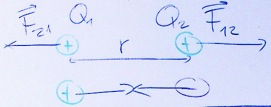
\includegraphics{Bild25}
\[ F_{21} = F_{12} = \frac{1}{4 \pi \epsilon_0} \frac{Q_1 Q_2}{r^2} \]
elektrische Feldkonstante $\epsilon_0 = \SI{8.85e-12}{\ampere\second\per\volt\metre}$

\subsubsection{Kraftgesetz zwischen zwei Atomen}
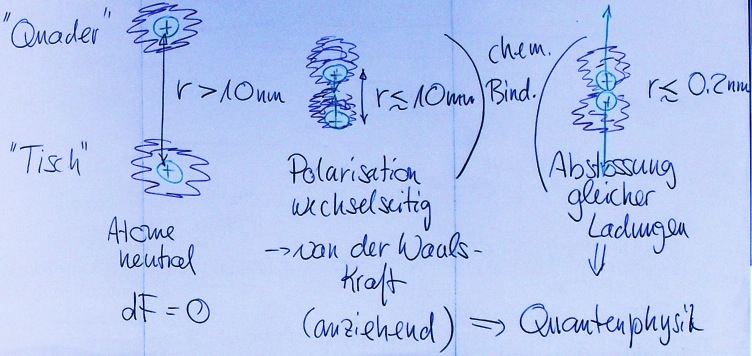
\includegraphics{Bild26}

\subsubsection{Kraftkurve}
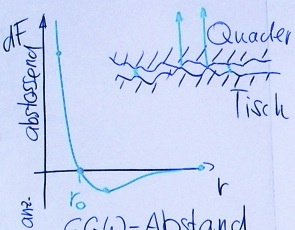
\includegraphics{Bild27} \\
GGW-Abstand (chemische Bindung)

\subsection{Reibungskräfte}
(parallel zur Berührungsfläche)

\subsubsection{Haftreibung}
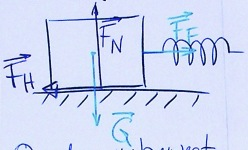
\includegraphics{Bild28} \\
Quader unbewegt \\
\[ \vec{F_H} = -\vec{F_F} \]

maximale Haftreibung:
\[ F_H \leq \underbrace{\mu_H}_{\text{Haftreibungszahl}} F_N \]

\subsection{Gleitreibung \texorpdfstring{$\vec{F_R}$}{F_R}}
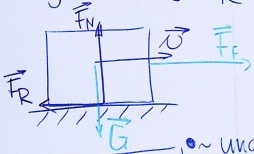
\includegraphics{Bild29}
\begin{itemize}
	\item Richtung: versucht immer Relativbewegung zu bremsen.
	\item unabhängig von $v$
\end{itemize}
\[ F_R = \mu_G \cdot F_N \]

\subsection{Kraftstösse}
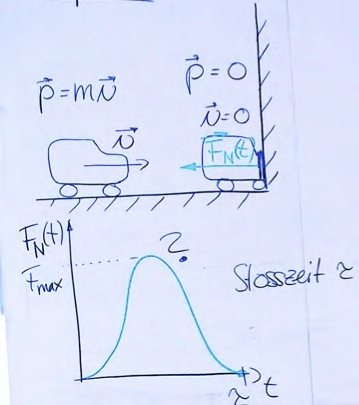
\includegraphics{Bild30}
\begin{rep*}
	Atomic Force Microscope (AFM) \\
	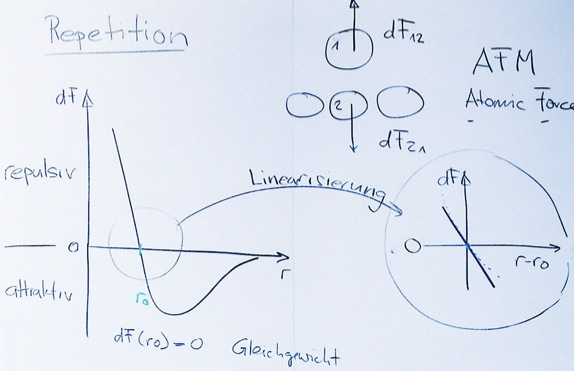
\includegraphics{Bild31}
	\[ \dd F =  -D ( r - r_0 ) = -\underbrace{D}_{\text{Federkonstante}} \cdot \underbrace{x}_{\text{Auslenkung}} \]
	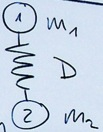
\includegraphics{Bild32}
	\[ D( \ce{O2} ) \approx \SI{1200}{\newton\per\metre} \]
\end{rep*}
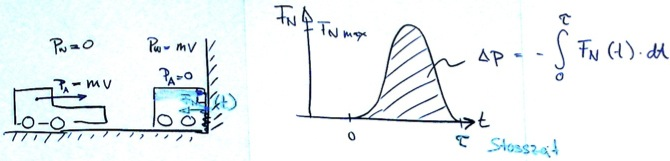
\includegraphics{Bild33}
\[ \Delta p = -\int_0^\tau F_n(t) \cdot \dd t \]
$\tau$ Stosszeit \\
kleine Kräfte $F_N$:
\begin{itemize}
	\item wenn $\tau$ gross
	\item wenn $\Delta p$ klein
\end{itemize}

\subsubsection{Experiment}
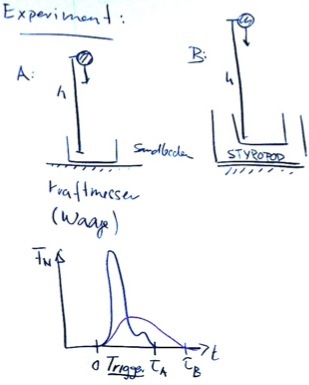
\includegraphics{Bild34}

\subsubsection{Vereinfachung}
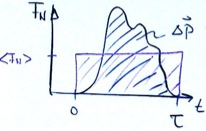
\includegraphics{Bild35}
\[ \Delta \vec{p} = m \vec{v} = - \scal{\vec{F_N}} \tau = - \int_0^\tau F_N(t) \dd t \]

\subsection{Das Drehmoment}
\begin{def*}[ note = Drehmoment , index = Drehmoment ]
	\[ \vec{M_0} = \vec{r} \times \vec{F} \]
\end{def*}
(Hebelgesetz) \\
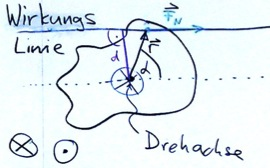
\includegraphics{Bild36}
\[ M_0 = r \cdot F_N \cdot \sin \alpha = \dd F_N \]
Rechte-Hand-Regel: \\
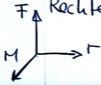
\includegraphics{Bild37}

\subsection{Gleichgewicht starrer Körper}
keine Bewegung:
\begin{gather*}
	\sum \vec{F_i} = 0 \quad \text{Translation} \\
	\sum \vec{M_i} = 0 \quad \text{Rotation}
\end{gather*}

\subsection{Der Schwerpunkt SP}
\begin{def*}[ note = Schwerpunkt , index = Schwerpunkt ]
	\[ \vec{r_s} = \frac{\sum \overbrace{m_i}^{\text{Massenelement}} r_i}{\sum m_i} \]
\end{def*}
gewichtetes  Mittel aller Orte der Körpermassen und ist der Angriffspunkt der Gewichtskraft \\
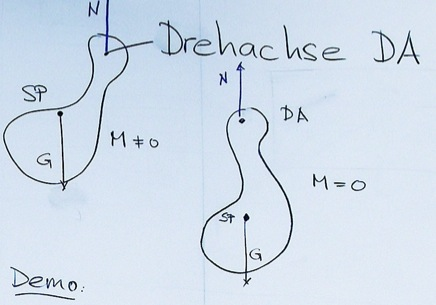
\includegraphics{Bild38}

\subsubsection{Denkexperiment Spazierstock}
Schwerpunkt des \\
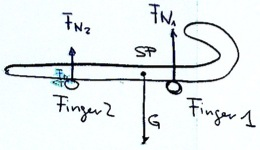
\includegraphics{Bild39} \\
wenn $F_{R_1} > F_{R_2}$ bewegt sich Finger 2.

\section{Festigkeitslehre (Elastizitätslehre)}
Reale Körper sind deformierbar (reversibel und/oder irreversibel). Festigkeit hängt vom Material und Form ab. \\
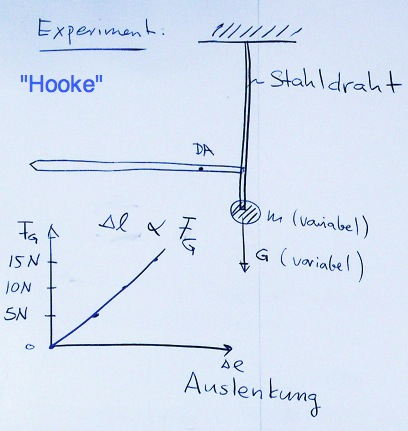
\includegraphics{Bild40}

\subsection{Materialverhalten}
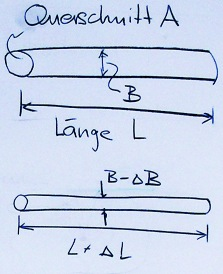
\includegraphics{Bild41} \\
\begin{def*}[ note = Dehnung , index = Dehnung ]
	\begin{gather*}
		\epsilon = \frac{\Delta L}{L} \\
		[ \epsilon ] = 1
	\end{gather*}
\end{def*}
\begin{def*}[ note = Querkontraktion , index = Querkontraktion ]
	\[ \beta = \frac{\Delta B}{B} \]
\end{def*}
\begin{def*}[ note = Normalspannung , index = Normalspannung ]
	\begin{gather*}
		\sigma = \frac{F_N}{A} \\
		[ \sigma ] = \si{\pascal}
	\end{gather*}
	Zugspannung $\sigma > 0$ \\
	Druckspannung $\sigma < 0$
\end{def*}

\subsubsection{Das Spannungs-Dehnungs Diagramm}
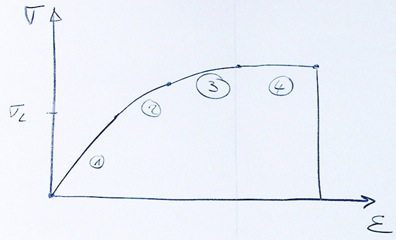
\includegraphics{Bild42} \\
\begin{enumerate}
	\item linearer Bereich $\sigma = E \epsilon$\footnote{$E$ Elastizitätsmodul, z.B. Stahl 200 GPa , Nanotubes 1TPa}
	\item nichtlinearer Bereich
	\item plastischer Bereich
	\item Fliessen
	\item Bruch
\end{enumerate}

\begin{rep*}
	\begin{itemize}
		\item Kraftstoss $\vec{F} \cdot \Delta t = \Delta \vec{p}$
		\item Derhmoment $\vec{M_o} = \vec{r} \times \vec{F}$ \\
			(Folien) \\
			gerichtete Grösse mit Drehsinn \\
			rechte Hand Regel \\
			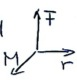
\includegraphics{Bild43}
		\item Schwerpunkt $\vec{r_{SP}} = \frac{\sum m_i \vec{r_i}}{\sum m_i}$
	\end{itemize}
	Festigkeitslehre \\
	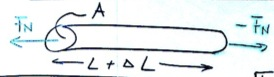
\includegraphics{Bild44} \\
	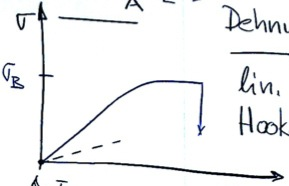
\includegraphics{Bild45}
	\begin{bsp*}
		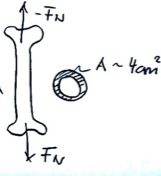
\includegraphics{Bild46}
		\[
			\sigma_{B \text{ Knochen}} = \SI{85}{\mega\pascal} \\
			\implies F_{N \text{ max}} = \sigma_B \cdot A = \SI{34}{\kilo\newton}
		\]
	\end{bsp*}
	Spannungs-Dehnungsdiagramm \\
	lin. Bereich Hooke'sches Gesetz:
	\[
		\sigma = \underbrace{E}_{\text{Elastizitätsmodul}} \cdot \epsilon \\
		\epsilon = \frac{\Delta L}{L} \quad []
	\]
\end{rep*}

\subsection{Scherung}
Demo: Schaumgummiquader \\
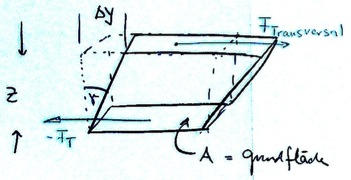
\includegraphics{Bild47} \\
Scherwinkel
\[ \gamma = \frac{\Delta y}{z} \]
\begin{def*}[ note = Schubspannung , index = Schubspannung ]
	\[
		\tau = \frac{F_T}{A} \\
		[ \tau ] = \si{\pascal}
	\]
	für den linearen Bereich (Hooke) gilt:
	\[ \tau = \underbrace{G}_{\text{Schubmodul } [ \si{\pascal} ]} \cdot \gamma \]
\end{def*}

\subsection{Spannungszustand}
Dehnung, Staucherung \\
Scherung, Biegung \\
Torsion \\
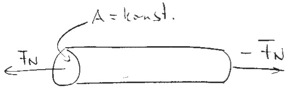
\includegraphics{Bild48} \\
Spannungsfelder
\[
	\sigma( x , y , z ) = \sigma(\vec{r}) = \frac{F_N}{A} = \text{ konst.} \\
	\tau(\vec{r}) = 0 \quad (\text{keine Scherung})
\]
Die Spannung in einem Körper lässt sich für jeden Punkt bestimmen.

\subsection{Die Biegebelastung eines Balkens}
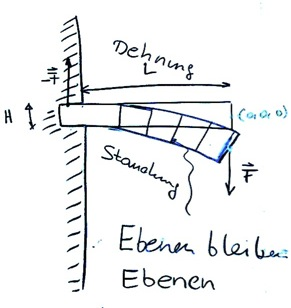
\includegraphics{Bild49} \\
Querschnitt $A = H \cdot B$ \\
Biegung:
\begin{itemize}
	\item $\sigma$ Normalspannung
	\item $\tau$ Schubspannungen
\end{itemize}
Problem: Bestimmung von $\sigma(\vec{r}) ; \tau(\vec{r})$ unter Berücksichtigung des Gleichgewichts

\subsubsection{Wahl des Koordinatensystems}
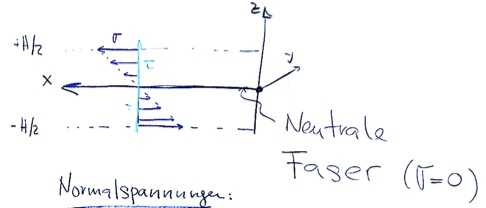
\includegraphics{Bild50} \\
Normalspannungen:
\[ \sigma( x , y , z ) = \alpha(x) \cdot z \]
prop. zur Dehnung. \\
Annahme: Gewichts des Balken $\ll F$ \\
Kräfte Gleichgewicht: \\
$z$-Komonente
\[ - F + A \cdot \tau(x) = 0 \implies \tau(x) = \frac{F}{A} = \text{ konst.} \]
$x$-Komponente:
\[
	\int_A \sigma( x , y , z ) \dd A = 0 \\
	\implies \int_{-\frac{H}{2}}^{+\frac{H}{2}} \alpha(x) \cdot z \cdot B \cdot \dd z = 0 \\
	\implies \alpha(x) \cdot B \underbrace{\int_{-\frac{H}{2}}^{+\frac{H}{2}} z \cdot \dd z}_{\text{muss $0$ sein}} = 0 \\
	\implies \text{ neutrale Faser liegt in der Mitte}
\]

\subsection{Drehmomentgleichgewicht}
\[
	\abs{M_\curvearrowright} = F \cdot x \\
	\abs{M_\curvearrowleft} = \int_A z \cdot \sigma( x , y , z ) \cdot \dd A \\
	\text{Gleichgewicht: } \abs{M_\curvearrowright} = \abs{M_\curvearrowleft} \\
	F \cdot x = \int_A z \cdot \alpha(x) \cdot z \cdot \dd A = \alpha(x) \cdot \underbrace{\overbrace{\int_A z^2 \dd A}^{\text{geometrischer Faktor}}}_{\text{Flächenträgheitsmoment } I_z} \\
	\implies \alpha( x , z ) = \alpha( x ) \cdot z = \frac{x \cdot z}{I_z} \cdot F
\]
Diskussion:
\begin{itemize}
	\item Neutrale Faser leigt bei $z=0$
	\item wo bricht der Balken bei $( L , y , \frac{H}{2} )$
	\item $I_z = \frac{1}{12} BH^3$ \\
		\includegraphics{Bild51}
\end{itemize}
\begin{rep*}[ note = Verteilung von Spannungen in festen Körper ]
	\begin{bsp*}[ note = Biegebelastung von Balken ]
		\includegraphics{Bild52} \\
		Koordinatensystem \\
		\includegraphics{Bild53} \\
		Querschnitt $A$ \\
		\includegraphics{Bild54}
		\[ I_z = \frac{1}{12} BH^3 \]
		Flächenträgheitsmoment $I_z$
		\[ \text{allg.:} \quad I_z = \int_A {\underbrace{z}_{\text{Abstand von $n$}}}^2 \dd z \]
	\end{bsp*}
\end{rep*}

\section{Hydrostatik}
\subsection{Der Hydrostatische Druck \texorpdfstring{$p$}{p}}
\begin{bsp*}[ note = Flüssigkeit ]
	\includegraphics{Bild55} \\
	\[
		\text{Druck } p = \frac{\sum \dd F}{A}  \\
		[ p ] = \frac{\text{N}}{\text{m^2}}
	\]
	Druck ist isotrop!
\end{bsp*}

\subsection{Der Luftdruck (Gase)}
\includegraphics{Bild56}

\subsubsection{Experiment: Bierglas}
\includegraphics{Bild57}

\subsubsection{Magdeburger Halbkugeln}
\includegraphics{Bild58}
\[
	p_L \approx 1 \text{bar} = 10^5 \text{Pa} \\
	A \approx 100 \text{cm}^2 \\
	F = p_L \cdot A = 10^3 \text{N} \approx 100 \text{kg}
\]

\begin{bsp*}[ note = Dehnung eines Blutgefässes ]
	\includegraphics{Bild59} \\
	\includegraphics{Bild60}
	\[
		\underbrace{p \cdot 2 \cdot R \cdot L}_{\color{Red}\downarrow\downarrow\downarrow} = \underbrace{2 \cdot \sigma \cdot d \cdot L}_{\color{Blue}\uparrow\uparrow} \\
		\implies \text{ Spannung } \sigma = \frac{R}{d} \cdot p \text{ mit } \epsilon = \frac{\sigma}{E} \\
		\implies V \text{ nimmt zu} \\
		\vdots \\
		\frac{\Delta V}{V} = \frac{2 \cdot R}{E \cdot d} \cdot \Delta p \eqqcolon \overbrace{D}^{\text{Dehnbarkeit}} \cdot \Delta p
	\]
\end{bsp*}

Physiologie oft:
\[
	\frac{\Delta V}{V} = \frac{\Delta p}{\underbrace{k}_{\text{Volumenelastizitätsmodul}}} \\
	k = \frac{1}{D}
\]

\subsubsection{Aneurysma}
\includegraphics{Bild61}
\[
	D = \frac{2R}{Ed} \\
	D' = \frac{2R'}{Ed'} > D \\
	\text{altendes Blutgefäss } E \nearrow \implies D \searrow
\]
$\implies$ krakhafte Gefässerweiterung

\begin{rep*}[ note = Hydrostatik ]
	hydrostatischer Druck in Flüssigkeiten / Gasen:
	\[ p = \frac{\sum \dd F}{A} \]
	\begin{itemize}
		\item isotrop!
		\item Luftdruck $p_0$
			\[ p_0 \approx 10^5 \text{Pa} = 1 \text{bar} \corresponds 1 \frac{\text{kg}}{\text{cm}^2} \text{!} \]
	\end{itemize}
	\begin{bsp*}[ note = Dehnung eines Gefässes ]
		\includegraphics{Bild62} \\
		$\implies$ Volumen
		\[
			V \rightarrow V + \Delta V \\
			\frac{\Delta V}{V} = \underbrace{\frac{2R}{Ed}}_{\text{Dehnbarkeit}} \cdot \Delta p
		\]
	\end{bsp*}
\end{rep*}

\subsubsection{Druckverteilung in Flüssigkeiten}
(auf Erdoberfläche) \\
\includegraphics{Bild63} \\
GGW
\[
	F_p( z_1 ) + G = F_p( z_2 ) \\
	F_p( = p \cdot A \\
	\implies p( z_2 ) = p( z_1 ) + \frac{G}{A} \\
	\implies p( z_2 ) = p( z_1 ) + \frac{( z_2 - z_1 ) \cdot \cancel{A} \cdot \rho \cdot g}{\cancel{A}} \\
	\text{Wähle } z_1 = 0 , z_2 = z \\
	p(z) = p_0 + z \cdot \rho \cdot g
\]

10m Wassertiefe
\[
	\rho \cdot g \cdot z = 10^3 \frac{\text{kg}}{\text{m}^3} \cdot 10 \frac{\text{m}}{\text{s}^2} \cdot 10 \text{m} = 10^5 \text{Pa} = 1 \text{bar} \\
	1 \text{mm} \ce{H20} \implies p = 9.8 \text{Pa} \\
	1 \text{mm} \ce{Hg} \implies p = 133 \text{Pa} \eqqcolon 1 \text{torr} \\
	\text{Blutdruck } \overline{p} \approx 100 \text{mm \ce{Hg}} = 133 \text{mbar}
\]

\subsubsection{Atmung beim Tauchen}
\includegraphics{Bild64}

\subsubsection{Luftdruck}
\[
	p_L(z) = ? \\
	\rho_L \approx 1 \frac{\text{kg}}{\text{m}^3} \\
	\rho_W \approx 10^3 \frac{\text{kg}}{\text{m}^3}
\]

\subsection{Der Auftrieb}
\includegraphics{Bild65}
\[
	F_{\text{res}} = F_p(z_1) + G - F_p(z_e) = G - ( p(z_2) - p(z_1) ) \cdot A = ( z_2 - z_1 ) A \cdot \rho_K \cdot g \underbrace{ - ( z_2 - z_1 ) A \cdot g \cdot \rho_{\text{Fl}}}_{F_A} \\
	F_{\text{res}} = \underbrace{( z_2 - z_1 )}_{V_K} \cdot A \cdot g ( \rho_K - \rho_{\text{Fl}} \\
	\rho_K > \rho_{\text{Fl}} = F_{\text{res}} > 0 \quad \downarrow \\
	\rho_K < \rho_{\text{Fl}} = F_{\text{res}} < 0 \quad \uparrow
\]

\subsubsection{Druckverteilung in Zentrifuge}
\includegraphics{Bild66} \\
$\implies$ Trennung von Stoffen durch Sedimentation $m$ auf Kreisbahn $\implies$ Zentripetalbeschleunigung $a_z$
\[
	a_z = \frac{v^2}{r} = r \omega^2
	\intertext{2.N.P $F_z = m a_z$ ; Rechnung:}
	\dots p(r) = p_0 + \frac{1}{2} \rho_{\text{Fl}} \omega^2 (r^2 - r_0^2)
	\intertext{Ultrazentrifuge 100000 $\frac{\text{U}}{\text{min}}$}
	\omega = 2\pi f = 10500 \text{s}^{-1} \\
	r \approx 5 \text{cm} \\
	\implies p \approx 1.3 \text{kbar}
\]
\includegraphics{Bild67}

\section{Energie und Arbeit}
\subsection{verschiedene Energieformen}
\begin{description}
	\item[kinetische Energie] BILD
		\[ E_{\text{kin}} = \frac{1}{2} m v^2 \]
	\item[potentielle Energie] BILD
		\[ E_{\text{pot}} = mgh \]
	\item[Federenergie] BILD
		\[ E_{\text{pot}} = \frac{1}{2} D x^2 \]
\end{description}

\subsection{Arbeit}
Umwandlung einer Energieform in die andere via Kräfte \\
\includegraphics{Bild68} \\
\begin{def*}[ note = Arbeit , index = Arbeit ]
	\[
		\begin{split}
			\dd W
				&= \vec{F} \cdot \vec{\dd r} \\
				&= F \cdot \dd r \cdot \cos \phi \\
				&= F_{||} \cdot \dd r
		\end{split}
		\intertext{Gesamte Arbeit}
		W_{1 \rightarrow 2} = \int_1^2 \vec{F} \cdot \vec{\dd r} \\
		[ W ] = \si{\newton\metre} = \si{\joule} \text{ (Joule)}
	\]
\end{def*}
\begin{bsp*}[ note = Arbeit zum Spannen einer Feder ]
	\includegraphics{Bild69} \\
	ganz langsam!
	\[
		\implies E_{\text{kin}} = 0 \\
		\vec{F_M} = -\vec{F_F} \\
		F_F = -D \cdot x \\
		\text{Arbeit der Hand } W_{0 \rightarrow x_0} = \int_0^{x_0} \vec{F_M} \cdot \vec{\dd r} \\
		W_{0 \rightarrow x_0} = \int_0^{x_0} F_M \cdot \dd x = \int_0^{x_0} D \cdot x \dd x = \left. \frac{1}{2} D x^2 \right|_0^{x_0} = \frac{1}{2} D x_0^2
	\]
\end{bsp*}

\begin{rep*}[ note = Hydrostatik ]
	Druckverteilung in Flüssigkeiten:
	\[ p(z) = p_0 + \rho_{\text{Fl.}} g z \]
	\includegraphics{Bild70}
	\begin{folge}[ note = Auftrieb ]
		\includegraphics{Bild71}
	\end{folge}
	Zentifuge:
	\[ p(r) = p_0 + \frac{1}{2} \rho_{\text{Fl.}} \omega^2 ( r^2 - r_0^2 ) \]
	Energie und Arbeit: \\
	\includegraphics{Bild72} \\
	Arbeit:
	\[ W_{1 \rightarrow 2} = \int_1^2 \vec{F} \cdot \vec{\dd r} \]
	z.B. Spannen einer Feder
	\[ W_{0 \rightarrow x_0} = \frac{1}{2} D x_0^2 \]
\end{rep*}

\subsection{Energie und Energieerhaltungssatz}
\subsubsection{Situation}
\includegraphics{Bild73} \\
$W_{1 \rightarrow 2}$: Arbeit sämtlicher an $m$ angreifender Kräfte ($\vec{F_{\text{res}}}$)
\[ W_{1 \rightarrow 2} = \int_1^2 \vec{F_{\text{res}}} \cdot \vec{\dd r} \]
\begin{satz*}[ note = Energiesatz , index = Energie satz Satz , indexformat = {1!~.2 3!1~} ]
	\[ W_{1 \rightarrow 2} = E_{\text{kin}}^{(2)} - E_{\text{kin}}^{(1)} \]
\end{satz*}
\includegraphics{Bild74}
\begin{bsp*}[ note = Bremsung ]
	\includegraphics{Bild75}
	\[
		\vec{F_{\text{res}}} = \underbrace{\vec{G} + \vec{F_N}}_{0} + \vec{F_R} \\
		W_{1 \rightarrow 2} = -\int_0^L F_R \dd x = -\int_0^L \mu_G m g \dd x = -\mu_G m g L = 0 - \frac{1}{2} m v_0^2 \\
		L = \frac{v_0^2}{2 \mu_G g}
	\]
\end{bsp*}

\subsubsection{Situation Energieerhaltungssatz}
Bewegungen unter Einfluss \textbf{konservativer Kräfte} (z.B. Gewichtskraft , Federkraft ) \\
\includegraphics{Bild76} \\
$W_1$: Arbeit der \textbf{konservativen} Kraft \\
\textbf{konservativ}: $W_1 = W_2 = W_3$ ; $W_{1 \rightarrow 2}$ ist unabhängig vom Weg \\
$\implies$ zwei Zahlen (bei Ort 1,2 genügen) \\
$\implies$ $W_{1 \rightarrow 2}$ hängt nur von Lage ab
\begin{def*}[ note = potentielle Energie , index = potentielle Energie , indexformat = {2!1~}]
	\[ E_{\text{pot}}^{(2)} - E_{\text{pot}}^{(1)} = - W_{1 \rightarrow 2} \]
\end{def*}
\begin{bsp*}
	\includegraphics{Bild77}
	\[
		E_{\text{pot}}^{(1)} = mgh \\
		E_{\text{pot}}^{(2)} = 0 \\
		W_{1 \rightarrow 2} = \int_1^2 mg \dd z = mgh
		\intertext{Also:}
		0 - mgh = -mgh \quad \checkmark
	\]
\end{bsp*}
\begin{satz*}[ note = Energie-Erhaltungssatz , index = Energie-Erhaltungs satz Satz , indexformat = {1!~.2 3!1.~} ]
	\[ E_{\text{tot}} = E_{\text{kin}} + E_{\text{pot}} = \text{ konst.} \]
\end{satz*}
\begin{bsp*}[ note = Berg- \& Talbahn ]
	\includegraphics[ width = \textwidth ]{Bild78}
\end{bsp*}
\section{Hydrodynamik: Strömungen in Flüssigkeiten}
\subsection{Stationäre Strömungen}
\includegraphics{Bild79} \\
Geschwindigkeitsfeld
\begin{itemize}
	\item $\vec{v}(\vec{r})$ zeitlich konst. \\
		$\rightarrow$ stationär
	\item laminare Strömung \\
		( $\bar{v} > v_{\text{krit.}} \implies$ turbulente Strömung )
\end{itemize}
\begin{def*}[ note = Volumenstromstärke (Volumendurchfluss) , index = Volumenstromstärke Volumendurchfluss , indexformat = {1 2} ]
	\[ I_V = \frac{\Delta V}{\Delta t} text{ durch Querschnitt } A \]
	Zusammenhang mit $\vec{v}$ \\
	\includegraphics{Bild80} \\
	\[
		L = v \cdot \Delta t
		\intertext{in Zeit $\Delta t$}
		\Delta V = v \cdot A \cdot \Delta t \\
		\implies I_v = A \cdot v
	\]
\end{def*}

\subsection{Kontinuitätsgleichung}
\includegraphics{Bild81}
\[
	\text{hinein: } I_V^{(1)} = A_1 \cdot v_1 \\
	\text{hinaus: } I_V^{(2)} = A_2 \cdot v_2 \\
	\implies A_1 v_1 = A_2 v_2
\]

\subsection{Die Bernoulligleichung}
Strömung unter Einfluss Druckkräften und Schwerkraft (keine Reibung!) \\
\includegraphics{Bild82} \\
Energiebilanz für Gewegung der Fl. \\
Arbeit $\Delta W$ (Druckkräfte) $- \Delta E_{\text{kin}} + \Delta E_{\text{pot}}$
\[
	\implies p_1 + \frac{1}{2} \rho v_1^2 + \rho g h_1 = p_2 + \frac{1}{2} \rho v_2^2 + \rho g h_2 \\
	\text{Gesamtdruck: } p_0 = p + \frac{1}{2} \rho v^2 + \rho g h  = \text{ statischer Druck } + \text{ dynamischer Druck } + \text{ Schweredruck}
\]

\begin{rep*}[ note = Strömungen in Flüssigkeiten ]
	Stationäre, laminare Strömungen \\
	\includegraphics{Bild83} \\
	Geschwindigkeitsfeld $\vec{v}(\vec{r})$ Zeitunabhängig
	
	Volumenstromstärke:
	\[ I_v = \frac{\Delta V}{\Delta t} = A \cdot v \]
	(wenn $\vec{v}(\vec{r})$ homogen sonst:
	\[ I_v = \iint_A \vec{v} \cdot \vec{\dd A} \]
	(Fluss-Integral))
	
	Kontinuitatsgleichung \\
	\[ A_1 v_1 = A_2 v_2 \]
	
	Bernoulli-Gleichung \\
	Entlang einer reibungsfreien laminaren Strömung gilt
	\[ \underbrace*{p}_{\text{Gesamtdruck}} = \underbrace*{p_0}_{\text{stat. Druck}} + \underbrace*{\frac{1}{2} \rho v^2}_{\text{dyn. Druck}} + \underbrace*{\rho g h}_{\text{Schweredruck}} \]
	(aus Energiesatz) $h$ nach oben!
\end{rep*}

\begin{bsp*}[ note = Hydrostatik ]
	(spez. $v \equiv 0$) \\
	\includegraphics{Bild84} \\
	BGl.:
	\[
		p_1 + 0 + \rho g \cdot 0 = p_2 + 0 + \rho g h \\
		\implies p_1 = p_2 + \rho g h
	\]
\end{bsp*}

\subsubsection{Druckmessung in Strömungen}
\includegraphics{Bild85}
\[ p = p_L + \rho g h \]
\begin{bsp*}[ note = Infusion ]
	\includegraphics{Bild86} \\
	BGl.:
	\[
		\cancel{p_L} + 0 + \rho g h = \cancel{p_L} + \frac{1}{2} \rho v_2^2 + 0 \\
		\implies v_2 = \sqrt{2gh}
	\]
\end{bsp*}

\subsubsection{Mariott'sche Flasche}
\includegraphics{Bild87}
\[ \implies v = \sqrt{2gh} = \text{ konst.} \]

\subsection{Innere Reibung}
reale Flüsigkeiten \\
\includegraphics{Bild88} \\
Konsequenz: \\
\includegraphics{Bild89} \\
Energiesatz: \\
\[
	\underbrace{\dd W}_{\text{Druckkräfte}} = \dd E_{\text{kin}} + \dd E_{\text{pot}} + \underbrace{\dd W_R}_{\text{innere Reibung}} \\
	\text{BGl: } p_1 + \frac{1}{2} \rho v_1^2 = p_2 + \frac{1}{2} \rho v_2^2 + \frac{\Delta F_R}{A}
\]
Kontinuitätsgleichung:
\[
	v_2 = v_1 \text{ !} \\
	\implies p_2 \neq p_1 ; p_2 - p_1 = \Delta p = -\frac{\Delta F_R}{A} \\
	\implies \text{ Druckabfall entlang Strömung}
\]

\subsection{Das Newtonsche Reibungsgesetz}
\includegraphics{Bild90} \\
Haften der Grenzschicht! \\
dynamische Schubspannung \\
Newtons Gesetz:
\[
	\tau = \eta \underbrace{\frac{\dd v}{\dd y}}_{\text{Geschwindigkeitsgefälle}} \\
	\eta \text{ Viskosität} \\
	[ \eta ] = \si{\pascal\second} \\
	1 \text{ Poise } = \SI{1}{\poise} = \SI{0.1}{\pascal\second}
\]

\subsubsection{Rohrströmungen}
\includegraphics{Bild91} \\
$\implies$ parabolische v-Verteilung \\
\includegraphics{Bild92}
Rechung:
\[
	v(r) = \frac{p_1 - p_2}{4 \eta L} (R^2 - r^2) \\
	\implies I_v = \iint_A \vec{v}(\vec{r}) \cdot \vec{\dd A}
\]

\subsection{Gesetz von Hagen-Poiseuille}
\[
	I_v = \frac{\pi R_4}{8 \eta L} (p_1 - p_2) \\
	I_v \sim R^4
\]
\begin{def*}[ note = Rohrwiderstand , index = Rohrwiderstand ]
	\[
		I_v = \frac{p_1 - p_2}{R_V} \\
		\implies R_V = \frac{8 \eta L}{\pi R^4}
	\]
\end{def*}

\subsubsection{Rohrsysteme}
\begin{bsp*}[ note = 2 Rohrstücke ]
	\includegraphics{Bild93} \\
	Serieschaltung
	\[ \implies R_V^{\text{Gesamt}} = R_V^{(1)} + R_V^{(2)} \]
	\includegraphics{Bild94}
\end{bsp*}

\begin{rep*}[ note = Hydrodynamik ]
	\includegraphics{Bild95} \\
	Innere Reibung $\implies$ Druckabfall $\Delta p$ entlang Strömung
	
	Newtonsches Reibungsgesetz \\
	\includegraphics{Bild96} \\
	dynamische Schubspannung
	\[ \tau = \eta \frac{\dd v}{\dd y} \]
	$\eta$: Viskosität
	\[ [ \eta ] = \si{\pascal\second} \]
	
	Rohrströmungen \\
	\includegraphics{Bild97}
	\[ I_v = \frac{\pi R^4}{8 \eta L} ( p_1 - p_2 ) = ( A \overline{v} ) \]
	
	Rohrwiderstand
	\[ I_v = \frac{p_1 - p_2}{R_v} \]
	( cf. $I = \frac{U}{R}$ )
	
	Gesetz von Hagen-Poiseuille \\
	Serie: \\
	\includegraphics{Bild98}
	\[ R_v^{\text{tot}} = R_v^{(1)} + R_v^{(2)} \]
\end{rep*}

\subsubsection{Parallelschaltung}
\includegraphics{Bild99}
\[ \implies \frac{1}{R_V^{\text{tot}}} = \frac{1}{R_V^{(1)}} + \frac{1}{R_V^{(2)}} \]

\subsection{Das Stokesche Reibungsgesetz}
\begin{bsp*}[ note = Kugel in Strömung ]
	\includegraphics{Bild100}
	\[ F_R = \underbrace{6 \pi R}_{\text{Kugel}} \eta v \]
\end{bsp*}

Anwedndung: Sedimentation \\
\includegraphics{Bild101} \\
2.N.P.
\[ ma = mg - m_{\text{Fl}} \cdot g - 6\pi R \cdot \eta \cdot v \]
Exp.
\[
	v = \text{ konst.} \implies a = 0 \\
	v_s = \frac{mg - m_{\text{Fl}} g}{6 \pi R \eta} \\
	v_s = \frac{\frac{4}{3} \pi R^3 (\rho_{K} - \rho_{\text{Fl}}}{6 \pi R \eta} \cdot g \\
	v_s = \frac{2}{9} \frac{( \rho_K - \rho_{\text{Fl}} )}{\eta} g R^2
\]

$\frac{\SI{50}{\milli\metre}}{\SI{30}{\minute}} \rightarrow$ Pferdeblut \\
\includegraphics{Bild102} WW zwischen Blutkörperchen \\
\begin{tabular}{ l l }
	Mann: &$\SIrange{3}{7}{\milli\metre\per\hour}$ \\
	Frau: &$7 - 11 \frac{\text{mm}}{\text{h}}$ \\
	Baby: &$1 - 2 \frac{\text{mm}}{\text{h}}$
\end{tabular}

\subsection{Turbulente Stömungen}
\includegraphics{Bild103} \\
$\frac{\Delta v}{\Delta y}$ grösser $\implies$ \\
\includegraphics{Bild104} \\
Wirbelbildung

\subsubsection{Rohrströmung}
\includegraphics{Bild105} \\
$\frac{\Delta v}{\Delta y}$ gross \\
Ab wann Turbulenz? \\
Reynoldsche Zahl $Re$
\[ Re = \frac{2R\rho}{\eta} \cdot \underbrace{\overline{v}}_{\text{mittlere Strömungsgeschwindigkeit}} \]

\subsubsection{Turbulenzkriterium}
\[ Re \gtrsim \underbrace{2300}_{\text{zyl. Röhre}} \]
kritische Geschwindigkeit $v_{\text{krit}}$
\[ Re = \frac{2R\rho}{\eta} \underbrace{\overline{v}}_{v_{\text{krit}}} = 2300 \]

\begin{bsp*}[ note = Blutströmung ]
	mittlere Strömungsgeschwindigkeit $\overline{v}$
	\[
		\text{H.P: } I_V = \frac{\pi R^4}{8 \eta L} \Delta p = A \overline{v} = \pi R^2 \overline{v} \\
		\overline{v} = \frac{R^2}{8 \pi L} \Delta p
	\]
	Blut: $\rho = 10^3 \frac{\text{kg}}{\text{m}^3} ; \eta \approx 4 \cdot 10^{-3} \text{Pa} \cdot \text{s}$ \\
	Aorta:
	\[
		\left. \begin{matrix*}[l]
			R &\approx 1 \cdot 10^{-2} \text{m} \\
			L &\approx 0.4 \text{m} \\
			\Delta p &\approx 40 \text{Pa}
		\end{matrix*} \right\} \begin{matrix*}[l]
			\overline{v} = 0.3 \frac{\text{m}}{\text{s}} \\
			Re = 1500
		\end{matrix*} \implies
	\]
	\includegraphics{Bild106}
\end{bsp*}

\subsubsection{Kapillare}
\[
	\left. \begin{matrix*}[l]
		R &\approx 4 \cdot 10^{-6} \text{m} \\
		L &\approx 0.001 \text{m} \\
		\Delta p &\approx 10^3 \text{Pa}
	\end{matrix*} \right\} \begin{matrix*}[l]
		\overline{v} = 5 \cdot 10^{-4} \frac{\text{m}}{\text{s}} \\
		Re = 0.001
	\end{matrix*} \implies \text{ nie Turbulent}
\]

\begin{rep*}[ note = Hydrodynamik ]
	Das Stoke'sche Reibungsgesetz \\
	\includegraphics{Bild107}
	\[ F_R = 6 \pi R \eta v \]
	
	Turbulente Strömung \\
	Reynoldszahl $Re = \frac{2R \cdot \rho}{\eta} \overline{v}$ \\
	Turbulenzkriterium: $\overline{v} \gtrsim v_{\text{krit}}$ \\
	Rohrströmung: $Re \gtrsim 2300$
\end{rep*}

\chapter{Thermodynamik (Wärmelehre)}
Gesetz der Mechanik angewandt auf sehr viele Teilchen

\section{Modell des idealen Gases}
\includegraphics{Bild108} \\
$N$ teilchen \\
ideales Gas
\begin{itemize}
	\item Teilchen punktförmig
	\item WW nur während Stössen
\end{itemize}
$m_i , \vec{r_i}(t) , \vec{v_i}(t) \implies$ vollständige Beschreibung \\
$\implies$ ist irrelevant (unmöglich bei $N \approx 10^{23}$ ) \\
TD: Wichtige Grössen des gesamten Gases, die sich zeitlich nicht ändern!

\subsection{Zustandsgrössen}
\begin{description}
	\item[Innere Energie]
		\[ U = \sum_{i = 1}^N \frac{1}{2} m_i v_i^2 \overset{!}{=} \text{ konst.} \]
		Wieso? \\
		\includegraphics{Bild109} \\
		Einzelstösse erhalten kinetische Energie!
	\item[mittlere Energie pro Teilchen]
		\[ \overline{E_{\text{kin}}} = \frac{1}{2} \overline{mv^2} = \frac{U}{N} \]
\end{description}

\subsection{Die Geschwindigkeitsverteilung}
Nicht alle Teilchen sind gleich schnell! \\
Zufallsbewegung, Stösse \\
$\implies$ Verteilung im Gas \\
\includegraphics{Bild110} \\
Histogramm! \\
$v_x$ ist Zufallsvariable \\
\includegraphics{Bild111} \\
Normalverteilung
\[ 
	n(v_x) = A_x e^{-\frac{v_x^2}{2\sigma^2}} \\
	v_x = \sigma \\
	n(\sigma) = A_x e^{-\frac{1}{2}} \approx 0.6 \cdot A_x
\]
$\implies$ $v_x$-Verteilung bleibt konstant, die einzelnen Teilchen änder dauernd $\vec{v}$. \\
$\implies$ Mittelwert $\overline{v_x} = 0$ \\
Wichtiger: Verteilung der Schnelligkeit
\[
	v = \sqrt{v_x^2 + v_y^2 + v_z^2} \geq 0
	\intertext{Resultat:}
	n(v) = A_v v^2 e^{-\frac{mv^2}{2kT}}
\]
\includegraphics{Bild112} \\
Maxwell-Boltzmann-Geschwindigkeitsverteilung \\
\includegraphics{Bild113}
\[ \implies \sigma^2 = \frac{kT}{m} \]

\subsection{Der Gasdruck}
Model \\
\includegraphics{Bild114} \\
Kraftstoss auf Wand:
\[ \Delta p_x = 2 m v_x = \int F_{TW} \cdot \dd t \]
\includegraphics{Bild115}
\[
	\Delta p_x = \overline{F_{TW}} \cdot \Delta t = \overline{F_{TW}} \cdot \frac{2L}{v_x} \\
	\overline{F_{TW}} = \frac{m v_x^2}{L}
\]
$N$ Teilchen \\
\includegraphics{Bild116} \\
$\implies$ Brownsche Bewegung \\
Druck $p$:
\[
	p = \frac{\overline{F_{TW}}}{A} \cdot N \cdot \underbrace{\frac{1}{3}}_{\text{Bewegung in $x$-Richtung}} \\
	p = \frac{1}{3} N \frac{m \overline{v}^2}{V} \\
	\overline{E_{\text{kin}}} = \frac{1}{2} m \overline{v}^2 \\
	\implies p = \frac{2}{3} \frac{N}{V} \overline{E_{\text{kin}}}
\]

\section{Temperatur}
\dots was ist das eigentlich? \\
All diese Grössen beschreiben einen bestimmten Zustand des Gases. \\
Zustandsänderungen (äussere Einwirkung) \\
$\implies$ Zustandsgleichung (ideales Gas) \\
Für $\SI{1}{\mole} = 6.02 \cdot 10^{23}$ Teilchen $= N_A$ (Avogadro-Konstante)
\[ p \cdot V = R \cdot T \]
$R$: universelle Gaskonstante
\begin{def*}
	\[ \SI{1}{\mole} \ce{^{12} C} \corresponds \SI{12.0}{\gram} \]
\end{def*}
\[ R = \SI{8.31}{\joule\per\mole\kelvin} \]
$T$ in Kelvin!
\begin{bsp*}[ note = {Volumen verringern ($T$ = konst.)} ]
	\[ p = \frac{RT}{V} \]
\end{bsp*}
\begin{bsp*}[ note = {Abkühlen ($p$ = konst.)} ]
	\[ V = \frac{R}{p} \cdot T \]
\end{bsp*}
Für $\nu$ mole:
\[ p \cdot V = \nu \cdot R \cdot T \]
Für Gasgemische:
\[
	\nu_1 , \nu_2 , \nu_3 , \dots \text{ mole} \\
	\implies pV = ( \nu_1 , \nu_2 , \nu_3 + \dots ) \cdot RT
\]
Partialdruck:
\[
	p_i = \nu_i \cdot \frac{RT}{V}
	\intertext{mit}
	p = p_1 + p_2 + p_3 + \dots
\]

\begin{rep*}[ note = Thermodynamik ]
	Modell des idealen Gases \\
	\includegraphics{Bild117} \\
	$N$ Teilchen ($10^{23}$!) \\
	$m_i , \vec{r_i}(t) , \vec{v_i}(t)$
	Zustand des Gases:
	\begin{itemize}
		\item Innere Energie
			\[ U = \sum_{i = 1}^N \frac{1}{2} m_i v_i^2 \]
		\item Mittlere kinetische Energie pro Teilchen:
			\[ \overline{E_{\text{kin}}} = \frac{U}{N} \]
		\item Gasdruck:
			\[ p = \frac{2}{3} \frac{N}{V} \overline{E_{\text{kin}}} \]
		\item Temperatur: \dots
		\item Maxwell-Boltzmann-Geschwindigkeitsverteilung \\
			\includegraphics{Bild118}
			\[ n(v) = A_v v^2 e^{-\frac{m v^2}{2kT}} \]
			Stellt sich durch Stösse ein!
	\end{itemize}
	
	Zustandsgleichung
	\[ p \cdot V = \underbrace*{\nu}_{\text{Anzahl Mole}} \cdot \underbrace*{R}_{\text{universelle Gaskonstante } = \SI{8.31}{\joule\per\mole\kelvin}} \cdot T \]
\end{rep*}

\subsection{Was ist Temperatur}
\begin{def*}[ note = thermodynamisches Gleichgewicht , index = thermodynamisches Gleichgewicht , indexformat = {12 2!1~} ]
	Zustandsgrössen sind zeitlich konstant
\end{def*}
\begin{bsp*}[ note = 2 Körper (auch Gase) ]
	\includegraphics{Bild119}
\end{bsp*}

\subsection{Wärmeaustausch}
\begin{itemize}
	\item Berührung (Wärmeleitung)
	\item Wärmestrahlung ($\rightarrow$ später)
\end{itemize}
$\rightarrow$ Temperaturmessung!

\subsubsection{Temperatur beim idealen Gas}
\[
	\SI{1}{\mole}: \\
	p \cdot V = RT \\
	p \cdot V = \frac{2}{3} N_A \overline{E_{\text{kin}}} \\
	\implies \overline{E_{\text{kin}}} = \frac{3}{2} \frac{R}{N_A} T = \frac{3}{2} \underbrace{k}_{\text{Boltzmann-Konstante} = \SI{1.38E-23}{\joule\per\kelvin}} T \\
	\implies \text{Temperatur $\approx$ Energie} \\
	\implies \overline{E_{\text{kin}}} = \frac{1}{2} \overline{m v^2} = \frac{3}{2} kT
\]

TD-GGW: weitere Situation
\section{Diffusion}
\begin{enumerate}
	\item \includegraphics{Bild120} \\
		$N$ Teilchen TD-GGW
	\item \includegraphics{Bild121} \\
		$t = 0$ \\
		Nicht-GGW, zeitlich veränderlich Diffusionsstromdichte $j_x$
	\item \includegraphics{Bild122} \\
		$t = \tau$ \\
		TD-GGW
\end{enumerate}

\subsection{Quantitative Beschreibung}
\includegraphics{Bild123} \\
alles gleiche Fläche \\
Teilchendichte $n(x)$ \\
zeitliche Änderung von $n(x)$ \\
Ursache: Dichtegefälle
\begin{enumerate}
	\item \[ n_1 = \frac{N}{V_1} \]
	\item \[ [ j_x ] : \si{Teilchen \per\metre\squared\second} \]
	\item \[ n_2 = \frac{N}{V} \]
\end{enumerate}
\[ j_x = -D \cdot \frac{\dd n}{\dd x} \]
Fick'sche Diffusionsgleichung \\
$D$: Diffusionskonstante
\[ [ D ] = \si{\metre\squared\per\second} \]
Man findet: $D \sim \underbrace*{\overline{l}}_{\text{mittlere freie Weglänge}} \cdot \underbrace*{\overline{v}}_{\text{mittlere Schnelligkeit}}$ \\
In Lösungen
\[
	\left. \begin{matrix*}[l]
		\text{Konzentration} \\
		c_i = \frac{\nu_i}{V_{\text{Lösg.}}}
	\end{matrix*} \right\} \quad j_x = -D \cdot \frac{\dd c_i}{\dd x}
\]

\subsection{Diffusion durch porösen Ton}
\includegraphics{Bild124} \\

\subsection{Gasaufnahme in Flüssigkeiten}
\includegraphics{Bild125} \\
Diffusion Gas $\rightleftarrows$ Flüssigkeitkeit \\
Gleichgewichtskonzentration $c_i^S$ (Sättigungskonzentration)

\subsubsection{Im TD-GGW}
\[ j_{gf} = j_{fg} \]
Prozesse:
$j_{gf}$: \includegraphics{Bild126} \\
$j_{gf} \sim n_{i,\text{gas}} \sim \underbrace{p_i}_{\text{Partialdruck}}$ \\
$j_{fg}$: \includegraphics{Bild127} \\
$\implies j_{fg} \sim c_i$ \\
$\implies c_1 \sim p_i$ \\
Henry-Dalton-Gesetz:
\[ c_i^S = K(T) \cdot p_i \]
$K(T)$: Gassorte, Flüssigkeit \\
$K(T) \searrow$ wenn $T \nearrow$

\section{Osmose}
Im TD-GGW \\
\includegraphics{Bild128} \\
Druck:
\[
	p \cdot V = \nu \cdot R \cdot T \\
	\implies p = \frac{\nu \cdot N_A \cdot k \cdot T}{V} = n \cdot kT \\
	\begin{split}
		\text{Druck }
			&\text{in } V_1 : p = n_\cdot \cdot kT + n_\bullet \cdot kT \\
			&\text{in } V_2 : p = n_\cdot \cdot kT
	\end{split} \\
	\implies \Delta p = n_\bullet kT \quad \text{osmotischer Druck (auch in Lösungen!)}
\]

\begin{rep*}[ note = Diffusion ]
	\includegraphics{Bild129}
	\[
		\begin{split}
			\text{Gase: } &j_x = -D \frac{\dd n}{\dd x} \\
			\text{Lösungen: } &j_x = -D \frac{\dd c}{\dd x}
		\end{split}
		\text{Konzentration } c_i = \frac{\nu_i}{V_{\text{Lösg}}}
	\]
	
	Diffusionskonstante
	\[ D \sim \underbrace*{\overline{l}}_{\substack{\text{hohe Dichte}\\\rightarrow \text{ langsam}}} \cdot \underbrace*{\overline{v}}_{\substack{\text{kleine Massen}\\\rightarrow \text{ Schnell}}} \]
	
	Gasaufnahme in Flüssigkeiten \\
	\includegraphics{Bild130}
	\[ c_i^S = K(T) \cdot p_i \]
	
	Osmose \\
	\includegraphics{Bild131}
	\[
		\begin{split}
			\text{Gase: } &\Delta p = n_\bullet \cdot kT \\
			\text{Lösungen: } &p_{\text{osm.}} = c_\bullet \cdot RT
		\end{split} \\
		\left( \text{aus } c_\bullet \cdot R = \frac{\nu}{V} R = \underbrace{\frac{\nu \cdot N_A}{V}}_{n_\bullet} k \right)
	\]
\end{rep*}

\section{Physiologische Kochsalzlösung}
\[
	c_{\text{physio}} = \SI{9}{\gram\per\litre} = \frac{\nu}{V_{\text{Lösg}}} \\
	\text{Molmasse: } m_{\ce{NaCl}} = \SI{23}{\gram} + \SI{35.5}{\gram} = \SI{58.5}{\gram} \corresponds 6.02 \cdot 10^{23} \ce{NaCl} \text{ Paare!} \\
	c = \frac{\SI{9}{\gram\per\litre}}{\SI{58.5}{\gram\per\mole}} \cdot 2 = \SI{0.308}{\mole\per\litre} = \SI{308}{\mole\per\metre\cubed} \\
	p_{\text{osm.}} = c \cdot R \cdot T = \SI{308}{\mole\per\metre\cubed} \cdot \SI{8.31}{\joule\per\mole\kelvin} \cdot \SI{310}{\kelvin} = \SI{7.93E5}{\pascal} \approx \SI{8}{\bar}
\]
Infusion mit reinem Wasser: Hämolyse \\
\includegraphics{Bild132}

\section{Der Dampfdruck}
ideales Gas $p = \frac{R \cdot T}{V}$ \\
\includegraphics{Bild133} \\
reales Gas \\
\includegraphics{Bild134} \\
\includegraphics{Bild135} \\
Dampfdruck-Kurve \\
\includegraphics{Bild136} \\
2 Situationen \\
Geschlossenes Gefäss (Kochtopf) \\
\includegraphics{Bild137} \\
Offenes Gefässe \\
\includegraphics{Bild138}

\section{Luftfeuchtigkeit}
absolute LF $f_a = \frac{m_{\ce{H2O}}}{V}$ in \si{\kilo\gram\per\metre\cubed} \\
relative LF $f_r = \frac{p_{\ce{H2O}}}{p_D(T)}$ in \% \\
$f_r = 100\% \implies$ Kondensation
\[ p_{\ce{H2O}} = \underbrace{\frac{m_{\ce{H2O}}}{M_{\ce{H2O}}}}_{\nu_{\ce{H2O}}} \cdot \frac{R \cdot T}{V} = f_a \cdot \frac{RT}{M_{\ce{H2O}}} \]

\section{1. Hauptsatz der Wärmelehre}
\includegraphics{Bild139} \\
Prozess: Man tut etwas mit dem System
\[ \Delta U = U_{\text{nach Prozess}} - U_{\text{vor Prozess}} = Q + W \]
Wie? z.B. Arbeit \\
\includegraphics{Bild140} \\
Gas leistet Arbeit $\implies W < 0$

\section{Wärmeleitung}
\includegraphics{Bild141} \\
Wie Diffusion!
\[ j_{wx} = -\lambda \cdot \frac{\dd T}{\dd x} \]
$\lambda$ Wärmeleitzahl [ \si{\watt\per\kelvin\metre} ] stark materialabhängig

\begin{bsp*}
	\includegraphics{Bild142}
	\[
		\lambda = \SI{0.1}{\watt\per\kelvin\metre} \\
		j_{wx} = \SI{-0.1}{\watt\per\kelvin\metre} \cdot \frac{\SI{20}{\kelvin}}{\SI{0.1}{\metre}} = \SI{20}{\watt\per\metre\squared}
	\]
\end{bsp*}
\begin{bsp*}[ note = \ce{H2O} ]
	\includegraphics{Bild143} \\
	$Q_S$: Schmelzwärme \SI{6.03}{\kilo\joule\per\mole} \\
	$Q_D$: Verdampfungswärme \SI{40.7}{\kilo\joule\per\mole}
	$\overset{Q > 0}{\implies} T_1 \overset{\tau}{\rightarrow} T_2$ \\
	$\Delta T = \frac{Q}{C}$ Wärmekapazität (des Systems) \\
	molare Wärekapazität $C_{\si{\mole}} = \frac{C}{\nu}$ [ \si{\joule\per\mole\kelvin} ] \\
	$Q$(Wasser von $\SI{0}{\celsius} \rightarrow \SI{100}{\celsius}$) $\approx \SI{8}{\kilo\joule\per\mole}$
\end{bsp*}

\begin{rep*}[ note = 1. Hauptsatz der Wärmelehre ]
	\[ \boxed{\Delta U = Q + W} \quad ( = Q^{\swarrow} + W^{\swarrow} ) \]
\end{rep*}

\begin{bsp*}[ note = \ce{H2O} ]
	\includegraphics{Bild144} \\
	Schmelzwärme $Q_S$ \\
	Verdampfungswärme $Q_D$ \\
	beides Umwandlungswärmen \\
	$\Delta U$:
	\begin{itemize}[ label = $\rightarrow$ ]
		\item Temeraturzunahme $\Delta T = \frac{Q}{C}$ ( $E_{\text{kin}} = \frac{3}{2} kT$ )
		\item Phasenumwandlung ( umgekehrt beim Ankühlen )
	\end{itemize}
	\includegraphics{Bild145}
\end{bsp*}

\section{2. Haupsatz der WL}
\includegraphics{Bild146} \\
\begin{bsp*}
	Wasserfall
\end{bsp*}
\textbf{Prozess ist irreversibel!}

2. HS: Welcher Anteil an ungeordneter Energie lässt sich wieder in geordnete Energie umwandeln?
\begin{def*}[ note = Entropie , index = Entropie S , indexformat = {1 2} ]
	\textbf{Entropie $S$} = Mass \textbf{für die Unordnung}
\end{def*}
Antwort: freie Energie $\boxed{F = U - TS}$

\chapter{Elekrizitätslehre}
zuerst Elektrostatik!

\section{Elektrostatik}
\subsection{Das Elektrische Feld}
\includegraphics{Bild147} \\
\[
	F_C = \frac{1}{4 \pi \epsilon_0} \frac{Q_1 Q_2}{r^2} \\
	\epsilon_0 = \SI{8.85E-12}{\ampere\second\per\volt\metre}
\]
\uline{hier:} \\
\includegraphics{Bild148}
\begin{def*}[ note = elektrische Feld , index = elektrische Feld , indexformat = {1!~2 2!1~} ]
	\[ \boxed{ \vec{E} = \frac{\vec{F_C}}{q} } \]
\end{def*}
\uline{hier:}
\[ E = \frac{1}{4 \pi \epsilon_0} \frac{Q}{r^2} \]
für Punktladung

\subsubsection{Feldlinien}
\begin{itemize}
	\item $\vec{E}$ tangential zu FL \\
		\includegraphics{Bild149}
	\item Richtungssinn!
	\item Dichte der FL $\sim \abs{\vec{E}(\vec{r})}$
	\item Vorzeichen: \\
		\includegraphics{Bild150}
\end{itemize}

\subsubsection{Mehrere Punktladungen}
\begin{bsp*}
	\includegraphics{Bild151} \\
	\uline{Vektoraddition!} \\
	\includegraphics{Bild152}
\end{bsp*}

\subsubsection{Das Dipolfeld}
\includegraphics{Bild153}
\begin{def*}[ note = Dipolmoment , index = Dipolmoment ]
	\[ \boxed{ \vec{p} = Q \cdot \vec{d} } \]
	\includegraphics{Bild154}
\end{def*}

\subsubsection{Dipol in äusserem Feld}
\includegraphics{Bild155} \\
\begin{itemize}
	\item Drehmoment
	\item Kraft (inhomogenes Feld)
\end{itemize}
\begin{bsp*}[ head = z.B. , note = \ce{H2O}-Molekül ]
	\includegraphics{Bild156}
\end{bsp*}

\subsubsection{Homogenes \texorpdfstring{$\vec{E}$}{E}-Feld}
\subsubsection{Plattenkondensator}
(kontinuierliche Ladungsverteilung) \\
\includegraphics{Bild157} \\
Im Innern:
\[ \boxed{ E = \frac{Q}{\epsilon_0 A} } \]
Aussen: $E \approx 0$

\subsection{Die Elektrische Spannung}
\includegraphics{Bild158} \\
Arbeit von \uline{mir}
\[
	W_{1 \rightarrow 2} = \int_{z_1}^{z_2} \vec{F} \cdot \vec{\dd r} = q E ( z_2 - z_1 ) > 0 \\
	( \vec{F} = - \vec{\overline{F_E}} = - q \vec{E} = \text{ konst. } )
\]
\begin{def*}[ note = elektrische Spannung , index = elektrische Spannung , indexformat = {1!~2 2!1~} ]
	\[
		\boxed{ U_{21} = \frac{W_{1 \rightarrow 2}}{q} }
		\intertext{( = Arbeit / Ladung )}
		[ U ] = \si{\joule\per\coulomb} = \si{\volt}
	\]
\end{def*}

\begin{rep*}[ note = Die elektrische Spannung ]
	\includegraphics{Bild159} \\
	\[
		\vec{E}(\vec{r}) \text{ hier homogen} \\
		\text{Probeladung } q \\
		\text{Arbeit } W_{1 \rightarrow 2} = \int_{z_1}^{z_2} \underbrace{\vec{F}}_{\text{\enquote{meine Kraft} } \vec{F} = - \vec{F_E} = - q \cdot E} \cdot \vec{\dd r} = q \cdot E ( z_2 - z_1 )
	\]
	\begin{def*}[ note = Spannung , index = Spannung ]
		\[ U_{21} = \frac{W_{1 \rightarrow 2}}{q} \]
	\end{def*}
\end{rep*}

konservatives Kraftfeld
\begin{itemize}[ label = $\implies$ ]
	\item $W_{1 \rightarrow 2}$ unabhängig vom Weg
	\item $W_{1 \rightarrow 2} = E_{\text{pot}}(z_2) - E_{\text{pot}}(z_1)$
\end{itemize}
Das \textbf{elektrische Potential}
\[ \boxed{ \phi(x) = \frac{E_{\text{pot}}(z)}{q} } \]
$\implies U_{21} = \phi(z_2) - \phi(z_1)$ \\
Spannung = Potenitaldifferenz
\begin{bsp*}
	hier $W_{1 \rightarrow 2} > 0$ \\
	$z_2$ liegt auf höherem Potential
\end{bsp*}

\subsection{Bewegung \texorpdfstring{$\perp$}{senkrecht zum} \texorpdfstring{$\vec{E}$}{E}-Feld}
\includegraphics{Bild160}
\[ \begin{split}
	W_{1 \rightarrow 2}
		&= \int_{x_1}^{x_2} \vec{F} \cdot \vec{\dd r} = 0 \\
		&= U_{21} = 0 \\
		&= \phi(x_2) - \phi(x_1)
\end{split} \]
\begin{bsp*}[ note = Plattenkondensator ]
	\includegraphics{Bild161}
	\[ U_{21} = - \frac{qEd}{q} = \underbrace{Ed}_{E = \frac{Q}{\epsilon_0 A}} = \frac{Qd}{\epsilon_0 A} \]
	\includegraphics{Bild162}
	\[ U_{21} = U \implies E = \frac{U}{d} \quad \left[ \si{\volt\per\metre} \right] \]
\end{bsp*}
\begin{def*}[ note = Kapazität , index = Kapazität ]
	\[ C = \frac{Q}{U} \]
	
	\[ \text{Plattenkondensator } C = \frac{\epsilon_0 A}{d} \]
\end{def*}

\subsubsection{Beliebiges \texorpdfstring{$\vec{E}$}{E}-Feld}
\includegraphics{Bild163}
\[ \begin{split}
	U_{21}
		&= \phi(2) - \phi(1) \\
		&= \frac{W_{1 \rightarrow 2}}{q} \\
		&= - \int_{1}^{2} \vec{E}(\vec{r}) \vec{\dd r}
\end{split} \]

\subsubsection{Beschleunigung in Röntgenröhre}
\includegraphics{Bild164}
\[
	\left. \begin{matrix*}[l]
		\phi(2) > \phi(1) \\
		q = -e
	\end{matrix*} \right\} \quad E_{\text{pot}}(2) < E_{\text{pot}}(1) \\
	\text{EEH: } -e \phi(1) + \underbrace{\frac{1}{2} m v_1^2}_{0} = -e \phi(2) + \frac{1}{2} m v_2^2 \\
	\implies \frac{1}{2} m v_2^2 = e ( \phi(2) - \phi(1) ) = e \cdot U_B
\]

\subsubsection{Materialien in elektrischen Feldern}
\subsubsection{Metalle}
\includegraphics{Bild165} \\
laden \\
\begin{tabular}{ l l }
	$+Q$ &Elektronen weg \\
	$-Q$ &Elektronen dazu
\end{tabular}

\subsubsection{Isolator}
\includegraphics{Bild166}

\subsubsection{Metalle}
Elektrostatik $\vec{v} = \vec{0}$
\begin{itemize}[ label = $\implies$ ]
	\item im Innern $\vec{E} = \vec{0}$
	\item Metalle sind Aequipotentialgebiete
\end{itemize}
\includegraphics{Bild167}

\subsubsection{Metall in äusserem Feld}
\includegraphics{Bild168} \\
Elektrometer \\
\includegraphics{Bild169}

\subsubsection{Isolator im äusseren Feld}
\includegraphics{Bild170}

\subsection{Elektrische Gleichströme: Leiter}
\includegraphics{Bild171} \\
\begin{itemize}[ label = $\implies$ ]
	\item $\phi(1) > \phi(2)$
	\item keine Aequipotentialfläche
\end{itemize}
$\vec{E}$-Feld beschleunigt Ladungen \\
Reibung an Ionen bremst sie \\
$\implies \vec{v} =$ konst.

\begin{rep*}[ note = Elekrische Spannung - elektrisches Potential ]
	\includegraphics{Bild172}
	\[ U_{21} = - \int_1^2 \vec{E} \cdot \vec{\dd r} \]
	\begin{bsp*}[ note = Punktladung ]
		\includegraphics{Bild173}
	\end{bsp*}
\end{rep*}

\includegraphics{Bild174}
\[ U_{21} = U \]
\begin{itemize}[ label = $\implies$ ]
	\item $\vec{E} \neq \vec{0}$ im Leiter
	\item Ladungsträger beschleunigt
\end{itemize}
+ Reibung $\implies$ $\vec{v} = $ konst. \\
\includegraphics{Bild175} \\
pos. Stromrichtung in Feldrichtung
\begin{def*}[ note = Stromstärke , index = Stromstärke ]
	\[ \boxed{ I = \frac{\increment Q}{\increment t} } \quad [ \si{\ampere} ] \]
\end{def*}
\begin{def*}[ note = Stromdichte , index = Stromdichte ]
	\[
		\boxed{ \vec{j} = \rho \cdot \vec{v} } \quad \left[ \si{\ampere\per\metre\squared} \right] \\
		\text{mit Ladungsdichte } \rho = \underbrace*{n}_{\text{Teilchendichte}} \cdot \underbrace*{z}_{\text{Ladung pro Teilchen}} \cdot \underbrace*{e}_{\text{Elementarladung } \approx \SI{1.6E-19}{\coulomb}}
	\]
\end{def*}

\subsubsection{Metalle}
i.A. Elektronen: $z = -1$

\subsubsection{Elektrolyt}
\[ \vec{j} = \vec{j_{+}} + \vec{j_{-}} = n_{+} z_{+} e \vec{v_{+}} + n_{-} z_{-} e \vec{v_{-}} \]
\begin{bsp*}[ head = z.B. ]
	\ce{Mg2+}-Ionen: $z = +2$
\end{bsp*}

In zylindrischem Leiter: \\
homogene Stromdichte \\
\includegraphics{Bild176}
\[ I = A j \implies j = \frac{I}{A} \]

\subsubsection{Inhomogenes \texorpdfstring{$\vec{j}(\vec{r})$}{j(r)}}
\begin{bsp*}[ note = Elektrolyt ]
	\includegraphics{Bild177}
	\[ I = \iint_A \vec{j} \cdot \vec{\dd A} \]
\end{bsp*}

\subsection{Strömungsgesetze}
\[ \begin{matrix*}[l]
	\text{\uline{Hyrdo:} } & I_V = \frac{p_1 - p_2}{\underbrace{R_V}_{\text{innere}\\\text{Reibung}}} \\
	\text{\uline{el. Strom:} } & I = \frac{U}{\underbrace{R}_{\text{Reibung}\\\text{an Ionen,}\\\text{Elektronen}}}
\end{matrix*} \implies \]
\begin{def*}[ note = elekrischer Widerstand , index = elektrischer Widerstand , indexformat = {12 2!1~} ]
	\[ \boxed{ R = \frac{U}{I} } \quad [ \si{\ohm} ] \]
	hängt ab von
	\begin{itemize}
		\item Material ($\rightarrow$ spez. Widerstand $\rho_W$)
		\item Form \\
			\includegraphics{Bild178}
			\[ R = \rho_W \frac{l}{A} \]
	\end{itemize}
\end{def*}

\subsection{Strom-Spannung-Charakteristik}
\subsubsection{Metall}
\includegraphics{Bild179} \\
\includegraphics{Bild180} \\
Steigung: $\frac{I}{U}$ \\
$\implies R = \frac{U}{I} = $ konst. \\
Ohmsches Gesetz

\subsection{Joulsche Wärme}
\includegraphics{Bild181} \\
$\vec{E}$-Feld leistet Arbeit (Batterie!)
\[ \dd W_{1 \rightarrow 2} = \dd Q \cdot U_{21} \]
$\implies$ \uline{elektrische Leistung}:
\[
	\boxed{ P = U \cdot I } \\
	P = \frac{\dd W_{1 \rightarrow 2}}{\dd t} = \underbrace{\frac{\dd Q}{\dd t}}_{I} \cdot U_{21} \\
	[ W ] = \si{\volt\ampere}
\]

\subsection{Elektrische Leitfähigkeit}
\[ I = \frac{1}{R} \cdot U \rightarrow \boxed{ \vec{j} = \sigma \cdot \vec{E} } \quad (\text{von } \vec{j} = \rho \cdot \vec{v}) \]
Bilanzgewinnung im ganzen Leiter \\
vektorielles Gesetz gilt überall im Leiter \\
\begin{def*}[note = elektrische Leitfähigkeit , index = elektrische Leitfähigkeit , indexformat = {12 2!1~} ]
	\[ \sigma = \frac{1}{\underbrace{\rho_W}_{\text{spez. Widerstand}}} \]
\end{def*}

\subsection{Elektrokardiogramm}
\includegraphics{Bild182}

\subsection{Spannungsquellen}
\begin{bsp*}[ note = Batterie ]
	\includegraphics{Bild183}
\end{bsp*}
\enquote{Elektromotorische Kraft} (EMK)
\[ E_m = \frac{W_{1 \rightarrow 2}}{q} \]
Leerlaufspannung $U_0 = E_m$
\begin{bsp*}[ note = Das Ruhepotential einer Zelle ]
	\includegraphics{Bild184} \\
	\includegraphics{Bild185}
	\begin{bsp*}
		\ce{K+}-Ionen \\
		innen Konz. $c_i$ \\
		aussen Konz. $c_a$ \\
		Im GGW sorgt Körper für $c_i > c_a$
		
		\uline{Lösung:} Konzentration in der Zellwand
		\[
			c(x) = c_i e^{-\frac{z e \cdot E \cdot x}{kT} }
			\intertext{am äusseren Rand}
			c(\delta) = c_a = c_i e^{-\frac{z e \cdot \overbrace{E \cdot \delta}^{\text{Diff. Spannung}}}{kT}}
			\intertext{Diff'spannung $U_D= E \delta$}
			\boxed{ U_D = \frac{kT}{z \cdot e} \ln \frac{c_i}{c_a} }
		\]
		Ruhepotential $U_D \approx \SI{90}{\milli\electronvolt}$
	\end{bsp*}
\end{bsp*}

\begin{rep*}[ note = El. Gleichströme ]
	\[
		\begin{matrix*}[l]
			\text{\uline{Stromstärke:} } &\boxed{ I = \frac{\increment Q}{\increment t} } \\
			\text{\uline{Stromdichte:} } &\boxed{ \vec{j} = \rho \cdot \vec{v} }
		\end{matrix*}
		\intertext{Strömungsgesetze:}
		\boxed{ I = \frac{U}{R} } \quad \boxed{ \vec{j} = \sigma \cdot \vec{E} }
	\]
	
	\uline{Spannungsquellen}
	\includegraphics{Bild186} \\
	$E_m$: elektromotorische \enquote{Kraft} \\
	$\implies$ Arbeit, um Ladung gegen E-Feld zu verschieben
	\begin{bsp*}[ note = Zellmembran ]
		\includegraphics{Bild187} \\
		$c_i > c_a$ \\
		\ce{K+}-Konzentration \\
		$\delta = \SI{5}{\milli\metre}$ \\
		Diffusion transportiert Ladungen (\ce{K+}) gegen E-Feld
		\[
			\implies U_D = \frac{kT}{ze} \ln \frac{c_i}{c_a} \\
			\text{Ruhepotential } \approx \SI{90}{\milli\volt} \\
			E = \frac{U_D}{\delta} = \frac{\SI{90E-3}{\volt}}{\SI{5E-9}{\metre}} = \SI{2E7}{\volt\per\metre}
		\]
	\end{bsp*}
\end{rep*}

\subsubsection{Reale Spannungsquellen}
\includegraphics{Bild188} \\
Innenwiderstand $R_i$
Spannungsabfall am $R_i$
\[ U_i = I \cdot R_i \]
Klemmanspannung
\[ U_{21} = E_m - I \cdot R_i = U_0 - I \cdot R_i \]
\includegraphics{Bild189} \\
\includegraphics{Bild190} \\
Kurzschluss:
\[ I_{\text{max}} = \frac{U_0}{R_i} \]

\subsection{Kirchhoffsche Maschenregel}
\[ \boxed{ \sum E_m = \underbrace{\sum U_i}_{\text{alle Spannungsabfälle}} } \]

\subsubsection{Kirchoffsche Knotenregel}
\includegraphics{Bild191} \\
Hier $I_1 = I_2 + I_3$
\[ \boxed{ \sum I_{\text{zufl.}} = \sum I_{\text{abfl.}} } \]
(Kontinuitätsgleichung)

\uline{Wichtig: Vorzeichen}
\includegraphics{Bild192} $E_M$ positiv \\
\includegraphics{Bild193} $I \cdot R$ negativ \\
\uline{Rezept:}
\begin{enumerate}[ label = \arabic*) ]
	\item Stromrichtungen einzeichnen (beliebig)
	\item Knotenregel anwenden
	\item Maschenregel anwenden
	\item Gleichungen nach $I_1 , I_2, \dots$ auflösen
\end{enumerate}

\chapter{Magnetfelder}
\section{Stabmagnet}
(Permanentmagnet) \\
$\rightarrow$ magn. Dipolmoment $\vec{p_m}$ \\
\includegraphics{Bild194} \\
\enquote{magn. Induktion} \\
\includegraphics{Bild195} $= \Downarrow \vec{p_m}$

\section{Magnetfeld eines el. Stromes}
\includegraphics{Bild196} \\
$\vec{B}$-Feldstärke
\[ \boxed{ B(r) = \frac{\mu_0 \cdot I}{2 \pi r} } \]
gerader leiter \\
\begin{itemize}
	\item $\vec{B}$-Feldlinien sind Kreise
	\item Drehrichtung: rechte Hand-Regel
	\item $\vec{B}$-Feldlinien sind immer geschlossen!
\end{itemize}
\[ [ B ] = \text{ Tesla } = \si{\tesla} = \si{\newton\per\ampere\metre} \]
magn. Feldkonstante
\[ \mu_0 = \SI{4\pi E-7}{\newton\per\ampere\squared} \]

\section{\texorpdfstring{$B$}{B}-Feld einer geraden Spule}
\includegraphics{Bild197} \\
\uline{Innen:} homogenes $B$-Feld, stark
\[ \boxed{ B = \frac{\mu_0 \overbrace{N}^{\text{Zahl der Windungen}} I}{L} } \]
aussen: schwaches Dipolfeld

\section{Die Lorentzkraft}
Nur auf \uline{bewegte} Ladungen!
\[ \boxed{ \vec{F_L} = q \cdot ( \vec{c} \times \vec{B} ) } \]
\includegraphics{Bild198} \\
Im Elektrolyten:
\includegraphics{Bild199}

\begin{rep*}[ note = Magnetfelder ]
	\includegraphics{Bild200} \\
	\includegraphics{Bild201} \\
	magn. Dipolmoment in $B$-Feld
	\begin{itemize}[ label = $\rightarrow$ ]
		\item Drehmoment ($\vec{p_m} \rightarrow \parallel \vec{B}$)
		\item Kraft in inhom. $B$-Feld
	\end{itemize}
	
	\uline{$B$-Felder von Strömen gerader Leiter} \\
	\includegraphics{Bild202} \\
	\begin{itemize}
		\item Kreisförmige Feldlinien
		\item rechte-Hand-Regel
		\item \[ \boxed{ B = \frac{\mu_0 I}{2 \pi r} } \]
	\end{itemize}
	
	\uline{Spule} \\
	\includegraphics{Bild203} \\
	\begin{itemize}
		\item im Innern homogen
		\item \[ \boxed{ B = \frac{\mu_0 N I}{L} } \]
	\end{itemize}
	
	\uline{Lorentzkraft} \\
	\dots auf bewegte Ladungen ($\vec{v}$)
	\[ \boxed{ \vec{F_L} = q ( \vec{v} \times \vec{B} ) } \]
	\includegraphics{Bild204}
\end{rep*}

\section{Elektrischer Leiter in \texorpdfstring{$B$}{B}-Feld}
\includegraphics{Bild205} \\
\[ \vec{\dd F_L} = -e ( \vec{v} \times \vec{b} ) \]
$\drsh$ in Tafel hinein \\
$\implies$ Kraft auf Leiter \\
Leiterstück, Länge $l$, Stromstärke $I$
\[ \boxed{ \vec{F_L} = I \cdot ( \underbrace{\vec{l}}_{\text{Richtung des Stromes } I} \times \vec{B} ) } \]

\begin{bsp*}[ note = Kraft zwischen zwei Leitern ]
	\includegraphics{Bild206} \\
	Rollenverteilung! \\
	$I_1$: felderzeugend \\
	$I_2$: Strom auf den Kraft wirkt \\
	(3.N.P.: Situation symmetrisch)
	\[
		F_L = I_2 \cdot l_2 \cdot B_1 \\
		B_1 = \frac{\mu_0 \cdot I_1}{2 \pi d} \\
		\implies F_L = \mu_0 \frac{I_1 I_2}{2 \pi d} l_2
	\]
	symmetrisch in $I_1 , I_2$
	\begin{bsp*}[ note = im Experiment ]
		\[
			I_1 = I_2 = \SI{140}{\ampere} \\
			d = \SI{1}{\centi\metre}
			\implies F_L = \SI{0.04}{\newton}
		\]
	\end{bsp*}
\end{bsp*}

\section{Das Induktionsgesetz}
Drahtsschleife: \\
\includegraphics{Bild207} \\
$U_{\text{ind.}}$: Induktionsspannung \\
Faradaysches Induktionsgesetz
\[ \boxed{ U_{\text{ind.}} = - \frac{\dd \Phi}{\dd t} } \]
$\Phi$: magnetischer Feldfluss \uline{durch die Schliefe} \\
\includegraphics{Bild208} \\
$\Phi = B \cdot A$
\uline{Hydro}: $I_V = v \cdot A$ \\
\includegraphics{Bild209} \\
\[ \Phi = \vec{B} \cdot \vec{A} = B \cdot A \cdot \cos \alpha \]
\begin{bsp*}[ head = z.B. ]
	\[ \alpha = \ang{90} \implies \Phi = 0 \]
\end{bsp*}

\subsection{\texorpdfstring{$B$}{B} inhomogen}
\includegraphics{Bild210} \\
\[ \Phi = \iint \vec{B} \cdot \vec{\dd A} = \iint B \cdot \cos \alpha \cdot \dd A \]

\subsection{Flussänderung}
\begin{itemize}
	\item Fläche $A$ ändern
	\item Winkel $\alpha$ ändern
\end{itemize} 

\chapter{Schwingungsvorgänge}
schwingfähiges System \\
\includegraphics{Bild211}

\section{Energiebetrachtung}
\includegraphics{Bild212} \\
\begin{itemize}
	\item gegeben durch Schwingsystem
	\item Anfangsbedingungen
\end{itemize}
harmonische Schwingung
\[ x(t) = \underbrace{x_0}_{\text{Amplitude}} \sin( \underbrace{\omega_0}_{\text{Kreisfrequenz}} t + \underbrace{\phi_0}_{\text{Phase}} ) \]
\includegraphics{Bild213}
\[
	E_{\text{tot}} = E_{\text{pot}} + E_{\text{kin}} = \text{ konst. } = W \\
	E_{\text{pot}} = \frac{1}{2} D x^2 \\
	E_{\text{kin}} = \frac{1}{2} m \dot{x}^2
\]
Kreisfrequenz $\omega_0$
\[ \text{(2.N.P.)} \quad \omega_o = \sqrt{\frac{D}{m}} \]
Schwingungsperiode $T$
\[ \boxed{ T = \frac{2\pi}{\omega_0} } \]
Frequenz $f = \frac{1}{T} = \frac{\omega_0}{2\pi}$

\begin{rep*}
	\uline{Das Induktionsgesetz} \\
	\includegraphics{Bild214} \\
	magn. Fluss
	\[ \Phi = \iint \vec{B} \cdot \vec{\dd A} \]
	Faraday's Induktionsgesetz
	\[ \boxed{ U_{\text{ind}} = -\frac{\dd \Phi}{\dd t} } \]
	
	\uline{Schwingungsvorgänge} \\
	\uline{harmonische Schwingung:}
	\[ \boxed{ x(t) = \underbrace*{x_0}_{\text{Amplitude}} \sin( \underbrace{\omega_0}_{\text{Kreisfrequenz}} t + \underbrace{\phi_0}_{\text{Phase}} ) } \]
	\begin{bsp*}[ note = Federpendel ]
		\[ \omega_0 = \sqrt{\frac{D}{m}} \]
	\end{bsp*}
	\uline{Energieerhaltung} \\
	\includegraphics{Bild215}
	\[ E_{\text{tot}} = E_{\text{kin}}(t) + E_{\text{pot}}(t) = \frac{1}{2} m \dot{x}^2(t) + \frac{1}{2} D x^2(t) = W = \text{ konst.} \]
\end{rep*}

\section{Gedämpfte Schwingung}
Energie geht durch Reibung verloren! \\
\includegraphics{Bild216}
\[
	\text{Amplitude } x_0(t) = x e^{-\frac{\delta}{2} t} \\
	x(t) = x_0 e^{-\frac{\delta}{2} t} \sin( \omega_d t + \phi_0 )
\]
schwache Dämpfung ($\delta$ klein) $\omega_d \approx \omega_0$
Energieverlust: $E_{\text{tot}} = E_{\text{pot}}( 0 ) \cdot e^{-\delta t}$

\section{Erzwungene Schwingung}
\includegraphics{Bild217} \\
periodische Anregung $F_0 \sin \omega t$ \\
2 Frequenzen!
\begin{itemize}
	\item ohne Anregung: $\omega_0 = \sqrt{\frac{D}{m}}$ Eigenfrequenz
	\item Anregungsfrequenz $\omega$ frei wählbar
\end{itemize}
Frage: Bewegung mit $\omega$ oder $\omega_0$? \\
Zu Beginn: Einschwingung mit $\omega_0$ (gedämpft) und $\omega$! \\
$t \rightarrow$ gross: stationärer Zustand. Nur noch $\omega$!

\subsection{Nur noch stationärer Zustand}
(mit Dämpfung: rasch im stationärem Zustand)
\[ \boxed{ x(t) = x_0(\omega) \cdot \sin( \omega t + \phi(\omega) ) } \]
\includegraphics{Bild218} \\
Anregung: $F_0 \sin \omega t$ \\
Resonanz:
\[ \boxed{ \omega_R \approx \omega_0 , \phi = -\frac{\pi}{2} , x_0 = \text{ maximal} } \]

\subsection{Erklärung der Phase bei Resonanz}
\includegraphics{Bild219}
\[ x(t) = x_0 \sin( \omega t - \frac{\pi}{2} = - x_0 \cos \omega t \]
$\implies$ Verschiebung $\vec{\dd r}$ \\
$\implies \vec{F_{AR}}$ verrichtet immer positive Arbeit!

\section{Anwendung: Magnetische Resonanztomographie (MRI)}
\subsection{Wasserstoffkern}
\includegraphics{Bild220} \\
\begin{itemize}
	\item Ladung $+e$
	\item Eigendrehimplus (Spin)
	\item magn. Moment $\vec{p_m}$
\end{itemize}
\subsection{\texorpdfstring{\ce{H}}{H}-Kerne in starkem Magnetfeld}
$\drsh$ magn. Moment $\vec{p_m}$ + Drehimpuls \\
\includegraphics{Bild221} \\
$\implies$ Präzessionsbewegung \\
\[
	\vec{B} = ( 0 , 0 , B_z )
	\intertext{Präzessions-(Larmor-)Frequenz}
	\boxed{ \omega_L = \gamma \cdot B_z }
\]
$\gamma$: gyromagn. Verhältnis \\
Wasserstoffkern: $\gamma = 2\pi \cdot \SI{42.58}{\mega\hertz\per\tesla}$

\subsection{Kernresonanz-Spektroskopie}
\includegraphics{Bild222} \\
Anregungsfrequenz $\omega$ \\
Resonanz $\omega = \omega_L$ \\
$\implies \vec{p_m}$ klappt herunter

\begin{rep*}[ note = Erzwungene Schwingung ]
	\uline{Anregung:} $F_0 \sin \omega t$ \\
	\uline{Schwingungssystem}, Eigenfrequenz $\omega_0$ \\
	$\implies$ stationärer Zustand:
	\[
		\boxed{ x(t) = x_0(\omega) \sin( \omega t + \phi(\omega) ) }
		\intertext{\uline{Resonanz:}}
		\boxed{ \begin{matrix*}[l]
			\omega_R \approx \omega_0 \\
			x_0( \omega_R ) \text{ maximal} \\
			\phi( \omega_R ) = -\frac{\pi}{2}
		\end{matrix*} }
	\]
	
	\uline{Kernresonanz-Spektroskopie (NMR)} \\
	\includegraphics{Bild223} \\
	\uline{\ce{H}-Kerne}:
	\begin{itemize}
		\item Drehmpuls
		\item magn. Moment
	\end{itemize}
	$\implies$ Präzision mit
	\[ \boxed{ \omega_L = \gamma B_z } \]
	\includegraphics{Bild224}
\end{rep*}

\subsection{Gradientenfeld \texorpdfstring{$\vec{B_z}(\vec{r})$}{B\textsubscript{z}(r)}}
genau kennen!

\begin{itemize}[ label = $\implies$ ]
	\item Messe $U_{\text{ind}}$ bei $\omega_L( \vec{B_z} )$
	\item erhalte $U_{\text{ind}}( \vec{B_z}( \vec{r} ) )$
	\item $n_H( \vec{r} )$
\end{itemize}

\section{Wellen}
Was braucht es?
\begin{itemize}
	\item \uline{Medium}:
		\begin{bsp*}[ head = z.B. , note = Federkette ]
			\includegraphics{Bild225}
		\end{bsp*}
		$\implies$ viele Schwingungssysteme, \enquote{\uline{Oszillatoren}} + Kopplung zwischen Oszillatoren \\
		Oszillatoren identisch $\implies$ resonante Ausbreitung
	\item \uline{Anregung} (=Welle): \enquote{Störung}, die sich im Medium ausbreitet \\
		$\implies$ Welle transportiert \uline{Energie}, nicht Masse!
\end{itemize}

\subsection{Polarisation}
= Bewegungsrichtung der einzelnen Oszillatoren \\
\uline{Pendel:} \\
\includegraphics{Bild226} \\
Wellenmaschine: \\
\includegraphics{Bild227}

\subsection{Ausbreitungsgeschwindigkeit \texorpdfstring{$c$}{c}}
\dots hängt ab von Medium (m,D)

\subsection{Mathematische Beschribung}
\[
	u( x , t ) = u( x - ct ) \quad ( \rightarrow \text{ pos. $x$-Richtg. } ) \\
	u( x , t ) = u( x + ct ) \quad ( \rightarrow \text{ neg. $x$-Richtg. } )
	\intertext{harmonische Wellen:}
	\begin{split}
		u( x , t )
			&= u_0 \sin( k ( x - ct ) ) \\
			&= u_0 \sin( \underbrace{k}_{\text{Wellenzahl } [ \si[ per-mode=reciprocal ]{\per\metre} ]} x - \underbrace{\omega}_{k \cdot c \\ \text{Kreisfreq.}} t ) \\
			&= u_0 \sin\left( \frac{2\pi}{\lambda} x - 2\pi \underbrace{f}_{\text{Frequenz}} \cdot t \right)
	\end{split}
\]

\subsection{Welle im Ortsbild}
\includegraphics{Bild228} \\
Zeit $t_0$ fest
\[ u( x , t ) = u_0 \sin( kx - \underbrace{\omega t_0}_{\text{konst. Phase}} ) \]
Wellenlänge $\lambda$
\[ \boxed{ \lambda = \frac{2\pi}{k} } \]

\subsection{Welle im Zeitbild}
\includegraphics{Bild229} \\
\uline{Ort $x_0$ fest} (1 Oszillator!)
\[
	u( x_0 , t ) = u_0 \sin( \underbrace{k x_0}_{\text{konst. Phase}} - \omega t ) \\
	\boxed{ T = \frac{2\pi}{\omega} }
\]

\subsection{Wichtiger Zusammenhang}
\[ c = \frac{\lambda}{T} = \lambda \cdot f \]
\uline{Schallwellen} (Akustik) \\
\uline{Medium}: Luft, Wasser, FK \\
\uline{Anregung} $u( x , t )$: longitudinale Auslenkung von Luftschichten \\
\includegraphics{Bild230}
\[ u( x , t ) = u_0 \sin( kx - \omega t ) \]
hier: $V' < V$ \\
Luft komprimiert!
\begin{def*}[ note = Schalldruck , index = Schalldruck ]
	\[ p_s( x , t ) = p( x , t ) - p_0 = - \underbrace{p_s^0}_{\text{Schalldruckamplitude}} \cos( kx - \omega t ) \]
\end{def*}

\uline{Ortsbild}: \\
\includegraphics{Bild231} \\
Schallgeschwindigkeit $c$ \\
\uline{Luft}:
\[ c = \sqrt{\frac{RT \kappa}{M}} = \sqrt{\frac{\frac{7}{5} p_0}{\rho}} \approx \SI{350}{\metre\per\second} \]

\subsection{Intensität}
\includegraphics{Bild232} \\
Energiestrom $I_E$ ( $\si{\joule\per\second} = \omega$ )
\[
	I_E = \underbrace*{\frac{1}{2} \rho}_{\text{kin. Energie pro Vol.}} \underbrace*{v_0^2}_{\text{\enquote{Schallschnelle}}} \cdot A \cdot c \\
	u( x , t ) \quad x = x_0 \\
	\implies v( x , t ) = \frac{\dd u( x , t ) }{\dd t} \\
	\text{Amplitude } v_0
	\intertext{\uline{Intensität}:}
	I = \frac{I_E}{A} = \frac{1}{2} \rho v_0^2 \cdot c = \frac{1}{2} \rho \omega^2 u_0^2 c \\
	\begin{bmatrix}
		u( x , t ) = u_0 \sin( kx - \omega t ) \\
		\implies v_0 = \omega \cdot u_0
	\end{bmatrix} \quad \dots \quad \boxed{ I = \frac{(p_s^0)^2}{2 \cdot \rho \cdot c} } \\
	\boxed{ I \sim u_0^2 }
\]

\subsection{Menschliches Ohr}
Hörschwelle $I_0 = 10^{-12}\si{\watt\per\metre\squared}$ \\
Schmerzgrenze $I_S \approx \SI{1}{\watt\per\metre\squared}$ \\
$\implies$ Wahrnehmung logarithmisch!

\subsubsection{Schallpegel}
\[ \boxed{ L = 10 \cdot \log_{10} \frac{I}{I_0} } \text{ in dezibel } \si{\deci\bel} \]
\begin{bsp*}
	\[
		I = I_0 \implies L = 0 \\
		\text{Schalldruckampl. } p_s^0 = \sqrt{2 \rho c I} = \SI{2e-5}{\pascal} = \SI{2e-10}{\bar}
	\]
\end{bsp*}

\begin{rep*}[ note = Harmonische Wellen ]
	\[ u( x , t ) = u_0 \sin( kx - \omega t ) \]
	$t = t_0$: \includegraphics{Bild233} \\
	\[
		\boxed{ k = \frac{2\pi}{\lambda} } \\
		\boxed{ \omega = 2 \pi f = \frac{2\pi}{T} } \\
		\boxed{ c = \frac{\lambda}{T} }
	\]
	
	\uline{Schallwellen} (in Gasen) \\
	$u( x , t )$: longitudinale Auslenkung von Luftschichten \\
	$p_s( x , t )$: \uline{Schalldruck} \\
	\uline{Schallgeschwindigkeit}
	\[ c = \sqrt{\frac{\frac{7}{5} p_0}{\rho}} \approx \SI{350}{\metre\per\second} \]
	\uline{Intensität}:
	\[ I = \frac{1}{2} \rho \omega^2 u_0^2 c = \frac{(p_s^0)^2}{2 \rho c} \]
	\uline{Schallpegel}:
	\[ \boxed{ L = 10 \cdot \log_{10} \frac{I}{I_0} } \text{ in \si{\deci\bel};  mit } I_0 = 10^{-12} \si{\watt\per\metre\squared} \]
	\begin{bsp*}[ head = z.B. ]
		\[
			L = \SI{80}{\deci\bel} \\
			80 = 10 \log \frac{I}{I_0} \implies 10^8 = \frac{I}{ 10^{-12} \si{\watt\per\metre\squared} }
		\]
	\end{bsp*}
\end{rep*}

\subsection{Hören von Schallwellen}
\begin{itemize}
	\item \uline{reiner Ton}: genau 1 Frequenz $f = \frac{\omega}{2\pi}$
		\[ \implies u( x , t ) = u_0 \sin( kx - \omega t ) \]
		Mittelohr: $x = x_0 = 0$ \\
		$\implies u_0 \sin \omega t \implies$ Frequenz $\rightcurvedarrow$ Ort der Anregung auf Kochlea
	\item \uline{Zwei Frequenzen}
		\[ u(t) = u_0 \sin\left( \frac{\omega_1 + \omega_2}{2} \right ) t \cdot \cos\left( \frac{\omega_1 - \omega_2}{2} \right) \]
		\uline{2 Fälle:}
		\begin{itemize}
			\item $\omega_1 , \omega_2$ stark verschieden \\
				\includegraphics{Bild234}
			\item $\omega_1 \approx \omega_2$ \\
				\includegraphics{Bild235}
				\[ \left. \begin{matrix*}[l]
					\implies \text{ mittlerre Frequenz } \frac{\omega_1 + \omega_2}{2} \\
					\implies \text{ Amplitude } 2 u_0 \cos\left( \frac{\omega_1 - \omega_2}{2} \right) t
					\end{matrix*} \right\} \quad \text{Schwebung}
				\]
		\end{itemize}
	\item \uline{Klang}: $u(t)$ ist periodische Funktion \\
		\includegraphics{Bild236}
	\item \uline{Geräusch}: $u(t)$ nicht periodisch \\
		\includegraphics{Bild237} \\
		\uline{Pistolenknall}: \\
		\includegraphics{Bild238}
\end{itemize}

\subsection{Ultraschall}
( $f \approx \SI{20}{\kilo\hertz} - \SI{100}{\mega\hertz}$ )

\subsubsection{Reflexion und Transmission}
\includegraphics{Bild239} \\
$M_1$: Luft \\
$M_2$: Wasser \\
\uline{Wellenwiderstand} $Z_W$
\[ \boxed{ Z_W = \rho \cdot c } \]
\includegraphics{Bild240} \\
Reflexion an inhomogenitäten im Blut ( $\implies$ bewegtes Medium ) \\
Erregung des Mediums (Blut)
\[ f' = f_0 \left( 1 + \frac{v_M}{c} \right) \]
(D.E. bei bewegtem Empfänger) \\
Erzeugt reflektierte Welle
\[ f^R = \frac{f'}{\left( 1 - \frac{v_M}{c} \right) } \]
(D.E. bei bewegtem Sender) \\
$\implies f^R \approx f_0 \left( 1 + 2 \frac{v_M}{c} \right)$ \\
$\implies$ \includegraphics{Bild241}

\begin{rep*}[ note = Elektromagnetische Wellen ]
	\includegraphics{Bild242} \\
	$\vec{E} \perp \vec{B}$ \\
	transversale Welle $E , B \perp$ Ausbreitung \\
	Ausbreitungsgeschwindigkeit: Vakuum \SI{3E8}{\metre\per\second}
	\[
		\boxed{ c = \lambda \cdot \upsilon } \\
		[ c ] = \si{\metre\per\second} \\
		[ \lambda ] = \si{\metre} \\
		[ \upsilon ] = \si[ per-mode = reciprocal ]{\per\second}
	\]
	\begin{bsp*}
		\[ \SI{100}{\mega\hertz} = \upsilon \implies \lambda = \SI{3}{\metre} \]
	\end{bsp*}
	
	Ausbreitungsmedium \\
	Vakuum und gewisse Materie z.B. Wasser, Glas, \dots \\
	\uline{Erzeugung}: beschleunigte Ladung \\
	Hertz'sche Dipol \\
	\includegraphics{Bild243}
\end{rep*}


\part{Anhänge}
\appendix

\chapter{Vorlesungsvorlagen}
\includepdf[pages={1-4},addtotoc={1,section,1,{Formelsammlung zur Hilfe beim Lösen der Übungsblättern und der Prüfung},formelsammlung}]{Formelsammlung_HS11}
\includepdf[pages={1},addtotoc={1,section,1,{Verteilung der Normalkräfte hängt von der Belastung ab. Beispiel Schuh},schuh}]{Schuh}
\includepdf[pages={1},addtotoc={1,section,1,{Das Drehmoment},drehmoment}]{Drehmoment}
\includepdf[pages={1},addtotoc={1,section,1,{Das Vektorprodukt, Rechte Hand Regel},vektorprodukt}]{Vektorprodukt}
\includepdf[pages={1},addtotoc={1,section,1,{Tabelle Elastizitätsmodule, Bruchspannungen},elastizitaetsmodule},landscape,angle=90]{Tabelle_Emodule_Bruchspann}
\includepdf[pages={1},addtotoc={1,section,1,{Bruchspannungen für Knochen},bruchspannungen},landscape,angle=90]{Bruchspann_Knochen}
\includepdf[pages={1},addtotoc={1,section,1,{Viskoelastische Materialien: Gummi und Muskel},gummimuskel}]{Gummi_Muskel}
\includepdf[pages={1},addtotoc={1,section,1,{Verformungen, Dehnung, Torsion},verformungen},landscape,angle=90]{Verformungen}
\includepdf[pages={1},addtotoc={1,section,1,{Fächenträgheitsmomente},flaechentraegheitsmomente},landscape,angle=90]{Flaechentraegheitsmomente}
\includepdf[pages={1},addtotoc={1,section,1,{Modell für Wirbelsäule - falsche Belastung},wirbelsaeule}]{Wirbelsaeule}
\includepdf[pages={1},addtotoc={1,section,1,{Torsion eines zylindrischen Stabes},torsion}]{Torsion}
\includepdf[pages={1},addtotoc={1,section,1,{Druckverteilung in der Atmosphäre, Barometerformel},barometerformel}]{Barometerformel}
\includepdf[pages={1},addtotoc={1,section,1,{Interatomare Kraft und deren Linearisierung - Federmodell},interatomarekraft}]{InteratomareKraft}
\includepdf[pages={1},addtotoc={1,section,1,{Von der interatomaren Kraft zur interatomaren potentiellen Energie},interatomarespotential}]{InteratomaresPotential}
\includepdf[pages={1},addtotoc={1,section,1,{Hagen-Poiseuille-Gesetz: Starke Abhängigkeit des Volumendurchflusses vom Rohr-Radius},rohrquerschnitte}]{Rohrquerschnitte}
\includepdf[pages={1},addtotoc={1,section,1,{Druckabfall entlang verzweigtem Rohrsystem},rohrverzweigung},landscape,angle=270]{Rohrverzweigung}
\includepdf[pages={1},addtotoc={1,section,1,{Druckverhältnisse in Infusionsgefäss/-leitung ohne und mit Kanüle},infusionen},landscape,angle=270]{Infusionen}
\includepdf[pages={1},addtotoc={1,section,1,{Schematische Darstellung des Kreislaufsystems},blutkreislauf},landscape,angle=90]{Blutkreislauf}
\includepdf[pages={1},addtotoc={1,section,1,{Zahlenmässige Charakterisierung des Kreislaufsystems},kreislauftabelle},landscape,angle=270]{KreislaufTabelle}
\includepdf[pages={1},addtotoc={1,section,1,{Verteilung des Druckabfalls im Kreislaufsystem},druckabfallkreislauf},angle=180]{DruckabfallKreislauf}
\includepdf[pages={1},addtotoc={1,section,1,{Blutdruckamplitude entlang des Kreislaufsystems},blutdruckamplitude},landscape,angle=270]{Blutdruckamplitude}
\includepdf[pages={1},addtotoc={1,section,1,{Strömung in Kapillaren: nicht-newtonsche Strömung},kapillarstroemung}]{Kapillarstroemung}
\includepdf[pages={1},addtotoc={1,section,1,{Maxwell-Boltzmannsche Geschwindigkeitsverteilung: Temperaturabhängigkeit},maxwellboltzmannvsT},landscape,angle=270]{MaxwellBoltzmannvsT}
\includepdf[pages={1},addtotoc={1,section,1,{Maxwell-Boltzmannsche Geschwindigkeitsverteilung: Massenabhängigkeit},maxwellboltzmannvsmasse},landscape,angle=270]{MaxwellBoltzmannvsMasse}
\includepdf[pages={1},addtotoc={1,section,1,{Gasaustausch in einer Lungen-Alveole},alveole}]{Alveole}
\includepdf[pages={1},addtotoc={1,section,1,{Dialysepatrone},dialysepatrone}]{Dialysepatrone}
\includepdf[pages={1},addtotoc={1,section,1,{Dampfdruckkurven von Wasser, Äthanol und Äther},sampfdruckkurven},landscape,angle=270]{Dampfdruckkurven}
\includepdf[pages={1},addtotoc={1,section,1,{elektrisches Dipolfeld},dipolfeld}]{Dipolfeld}
\includepdf[pages={1},addtotoc={1,section,1,{zwei ganz unterschiedliche Feldlinienbilder!},feldlinien}]{Feldlinien}
\includepdf[pages={1},addtotoc={1,section,1,{Dipole erzeugen Drehmomente und Kräfte auf andere Dipole},dipoleimdipolfeld}]{Dipole_im_Dipolfeld}
\includepdf[pages={1},addtotoc={1,section,1,{Hydratationsschale in wässrigen Lösungen},hydratation}]{Hydratation}
\includepdf[pages={1},addtotoc={1,section,1,{Kelvin-Generator},kelvingenerator}]{KelvinGenerator}
\includepdf[pages={1},addtotoc={1,section,1,{Der Mensch als elektrischer Leiter},menschalsleiter}]{MenschalsLeiter}
\includepdf[pages={1},addtotoc={1,section,1,{Bereiche der Wirkung elektrischer Ströme auf den menschlichen Körper},stromwirkungsbereiche},landscape,angle=270]{Stromwirkungsbereiche}
\includepdf[pages={1},addtotoc={1,section,1,{Schädigungen des Körpers durch elektrische Ströme},stromwirkung}]{Stromwirkung}
\includepdf[pages={1},addtotoc={1,section,1,{Ströme in der Elektro-Physiotherapie},physioelektroden},landscape,angle=270]{PhysioElektroden}
\includepdf[pages={1},addtotoc={1,section,1,{Zum Elektrokardiogramm (Figuren aus Kamke/Walcher)},ekg}]{EKG}
\includepdf[pages={1},addtotoc={1,section,1,{Zum Begriff der "elektromotorischen Kraft"},elektromotorischekraft}]{elektromotorischeKraft}
\includepdf[pages={1},addtotoc={1,section,1,{Schematisches Bild einer Zellwand},zellmembran}]{Zellmembran}
\includepdf[pages={1},addtotoc={1,section,1,{Beispiel für die Komplexität elektrischer Schaltkreise, Analogie zu Strömungen},kirchoffanalogie}]{KirchhoffAnalogie}
\includepdf[pages={1},addtotoc={1,section,1,{Beispiel zur Anwendung der Kirchhoffschen Regeln},kirchhoffnetzwerk}]{Kirchhoff_Netzwerk}
\includepdf[pages={1},addtotoc={1,section,1,{Parallel- und Serieschaltung von elektrischen Widerständen},widerstaende}]{Widerstaende}
\includepdf[pages={1},addtotoc={1,section,1,{Der Spannungsteiler},spannungsteiler}]{Spannungsteiler}
\includepdf[pages={1},addtotoc={1,section,1,{Sind magnetische Feldlinien tatsächlich immer geschlossen ? Magnetische Monopole ?},magmono}]{MagMono}
\includepdf[pages={1},addtotoc={1,section,1,{Der Wechselspannungsgenerator},wechselspannungsgenerator}]{Wechselspannungsgenerator}
\includepdf[pages={1},addtotoc={1,section,1,{Funktionsweise eines Fehlerstrom-Schutzschalters (FI)},fehlerstrom}]{Fehlerstrom}
\includepdf[pages={1},addtotoc={1,section,1,{Veranschaulichung der Kernspinresonanz},kernspinresonanz}]{Kernspinresonanz}
\includepdf[pages={1},addtotoc={1,section,1,{Schema eines Magnetresonanztomographen},mrtanlage}]{MRT-Anlage}
\includepdf[pages={1},addtotoc={1,section,1,{Magnetresonanztomographie: Kodierung des Ortes via Gradientenfeld},mriortfrequenz}]{MRIOrtFrequenz}
\includepdf[pages={1},addtotoc={1,section,1,{Magnetresonanztomographie: Aufnahme von Querschnitten},mriquerschnitt}]{MRIQuerschnitt}
\includepdf[pages={1},addtotoc={1,section,1,{Magnetresonanztomographie: Aufnahme von Längsschnitten},mrilaengsschnitt}]{MRILaengsschnitt}
\includepdf[pages={1},addtotoc={1,section,1,{Laufende Welle},laufendewelle},landscape,angle=90]{LaufendeWelle}
\includepdf[pages={1},addtotoc={1,section,1,{Ausbreitung von Schallwellen},schallwellen},landscape,angle=270]{Schallwellen}
\includepdf[pages={1},addtotoc={1,section,1,{Vergleich von Schallgeschwindigkeiten in verschiedenen Medien},schallgeschwindigkeiten}]{Schallgeschwindigkeiten}

\end{document}